\documentclass[twoside, a4paper, 12pt]{report}

\usepackage[inner=3cm, outer=3cm, a4paper]{geometry}
\usepackage{graphicx}
\usepackage{fancyhdr}
\usepackage{setspace}
\usepackage[american]{babel}
\usepackage{csquotes}
\usepackage[style=apa, backend=biber]{biblatex}

\pagestyle{fancy}

\renewcommand{\chaptermark}[1]{\markboth{#1}{}}

\fancyhf{} % clear the headers
\fancyhead[RO, LE]{%
   % The chapter number only if it's greater than 0
   \ifnum\value{chapter}>0 \chaptername\ \thechapter. \fi
   % The chapter title
   \leftmark}  
\fancyfoot[C]{\thepage}

\fancypagestyle{plain}{
  \renewcommand{\headrulewidth}{0pt}
  \fancyhf{}
  \fancyfoot[C]{\thepage}
}

\setlength{\headheight}{14.5pt}

\addbibresource{MiniProjectReport.bib}

\begin{document}
\begin{titlepage}
	\centering
	
\includegraphics[width=0.2\textwidth]{VeritasUniversityLogo}\par\vspace{1cm}
	{\scshape \LARGE Veritas University Abuja \par}
	{\scshape \Large (The Catholic University of Nigeria) \par}
	\vspace{1cm}
	{\huge Implementing a REST API for a Description of all Countries in the World Using Vue.js to Define the User Interface \par}
	\vspace{1.5cm}
	{\Large Ata, Chinonso Anita \par}
	{\Large VUG/CSC/17/1914 \par}
	\vspace{0.5cm}
	Submitted to \par
	\vspace{0.5cm}
	{\Large The Department of Computer and Information Technology College of Natural and Applied 			Sciences \par}
	\vspace{1cm}
	{\Large In Partial Fulfilment of the Requirement of Bachelors Degree of Computer Science \par}
	\vfill
	{\Large \today \par}
\end{titlepage}

\begin{abstract}
Abstract goes here...
\end{abstract}

\chapter*{Acknowledgements}
Acknowledgement goes here...

\pagenumbering{roman}
\tableofcontents
\listoffigures
\newpage
\pagenumbering{arabic}

\onehalfspacing

\chapter{Introduction}
\section{Motivation}
In the world today, having facts at your fingertips is very useful and important. With search engines like Google, life has been made easier as we do not have to visit libraries or spend money on books to get the most basic facts or knowledge. We now have all the information in the world in one place, and it is easy to gain access to it by just typing in a keyword or two and we have what we want.\\
\indent
What this application will do is to take this functionality further by putting all the countries in the world and their basic information such as their capital, population, continent, etc. in one place. Just like you would have in google, you could just go to the search box and type the name of any country in the world and you get information about that country that you're looking for.\\
\indent
As Technology is being incorporated in our everyday lives and things are being made easier each day it shouldn't stop us from still looking for ways to improve on these technologies to further make things easier in order to keep the world moving forward.

\section{Aims and Objectives}
By having a new interactive system that consists of a layout that displays all the countries in the world, the system can help users who just need quick and simple information about any country. It can also be used by students for assignments related to the subject and it can also be a fun way to learn about different countries in the world.\\
\indent
Thus, the application aims to produce a simple, interesting, and easy to use application that the user can refer to and rely on at anytime to give them the basic facts about any country in the world.\\
\indent
The objectives for developing the Rest Countries Application are as follows:
\begin{itemize}
\item To design a simple system and interface that can easily be viewed by any user to search for any country in the world and view simple information about the country that was searched for.
\item To develop a system that is accessible anywhere and on any device
\end{itemize}

\section{Features of the System}
The project is intended to produce an interactive system so that the user can feel interested to use the system. This this is achieved by implementing interactivity especially in the design of the system, a Graphical User Interface (GUI), and portability.

\subsection{Interactivity}
The definition of interaction is quite broad. \autocite{aoki2000taxonomy} stated that interactivity of a medium refers to a characteristic of communication settings a medium can create that allows users to interact.\\
\indent
Throughout the process of interaction design, the developer must be aware of key aspects in their design that influence emotional response in target users. The need for products to convey positive emotions and avoid negative ones is critical to any product success. These aspects include positive, negative, motivational, learning, creative, social and persuasive influences. A method that can be used to convey such aspects is the use of expressive interfaces. \autocite{kamari2011interactive} \\
\indent
In software, the use of of dynamic icons, animations and sound can help communicate a state of operation which in turn will create a sense of interactivity. Interface aspects such as fonts, colour palette, and graphical layouts can also influence an interface's perceived effectiveness.

\subsection{Graphical User Interface}
A graphical user interface (GUI) is a type of user interface item that allows people to interact with programs in more ways than typing. A GUI offers graphical icons, and visual indicators, as opposed to text-based interfaces, typed command labels or text navigation to fully represent the information and actions available to a user. The actions are usually performed through direct manipulation of the graphical elements.\\
\indent
There are several principles that need to be considered when dealing with a GUI.
\begin{itemize}
\item Layout\\
The interface should be a series of areas on the screen that are used consistently for different purposes.
\item Content Awareness\\
Users should always be aware of where they are in the system and what information is being displayed.
\item Aesthetic\\
Interface should be functional and inviting to users through careful use of white space, colours, and fonts. In this project for example, there is an option for the user to change the colour theme from light mode to dark mode and vice versa which makes the user feel like they are in control.
\item User Experience\\
The interface should be built in such a way that it is both easy to use and easy to learn. Novice users or infrequent users of software will prefer ease of learning and frequent users will prefer ease of use.
\item Consistency\\
Consistency in interface design enables users to predict what will happen before they perform a function. It is one of the important elements in ease of learning, ease of use, and aesthetic.
\end{itemize}

\subsection{Responsiveness}
The system is a full web application and this enables the system to be viewed anywhere no matter the device and the design is also fully responsive so the layout is still engaging whether the application is viewed on a small device or a very large device like a television. 

\chapter{Methodology}
\section{Introduction}
The system will be implemented using the waterfall model of system development life cycle as the project methodology. This methodology is selected because of its advantage which allows the requirements to be specified at the start of the project and for proper documentation.\\
\indent
The Waterfall Methodology is a linear approach to software development. It is also known as the 'Traditional Approach' because it is time-tested and easy to understand.\autocite{adenowo2013software}. The waterfall methodology breaks up the software development projects into steps: planning and analysis (Requirement Analysis), design and implementation, testing, system deployment, and maintenance. See Figure~\ref{fig:waterfall-methodology} for an illustration.

\begin{figure} [ht]
	\centering
	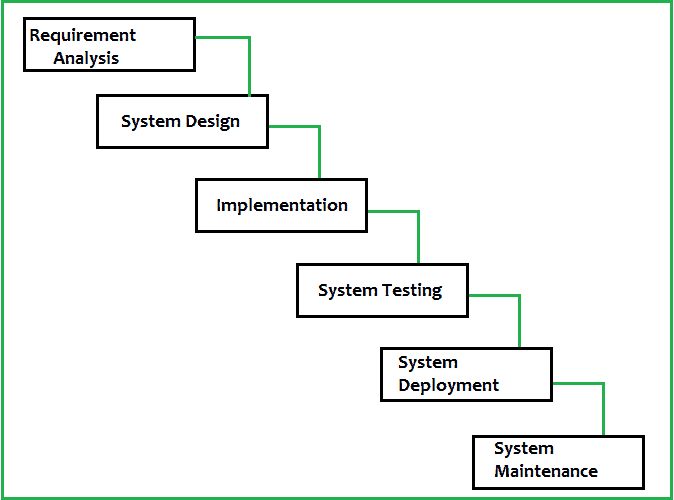
\includegraphics[width=1\textwidth]{waterfallmodelimg}
	\caption{Waterfall Methodology}
	\label{fig:waterfall-methodology}
\end{figure}

\section{Project Activities}

\subsection{Requirement Analysis}
In this phase, all the possible requirements of the system such as functional requirements, programming tools to be used, feasibility, and scope are captured and documented.\autocite{petersen2009waterfall}. The overall project is intended to come out with an interactive system that lets the user search for any country in the world and get information about that country.\\
\indent
At the beginning of the requirements analysis phase, the first thing that has been discussed is the programming tool that will be used which is Vue.js for the client-side, Node js with Express for the server-side and MongoDb for the database.

\subsection{Design and Implementation}
In the design phase, the actual database or file structure, user interface, system inputs and outputs is designed. Thereafter, the actual developement of the system takes place. A basic unit test is also conducted to verify that each component meets its requirement before handing the developed code over to the testing phase.

\subsection{Testing}
In this phase the system integration is tested regarding quality and functional aspects. In this case, the system will be tested by different users on their devices to make sure everything is working as it should. Furthermore, any response will be taken into consideration to improve the system in future.

\subsection{System Deployment}
In this phase when the application has been fully tested, the whole system will be transferred from development mode to build mode. The system will then be brought into shippable state. The database will be set up on MongoDb Atlas and the application itself will be deployed to Heroku.

\subsection{Maintenance}
After the product has been released, there might still be some problems in the user environment. Fixing those issues will require regular maintenance and patches to be released.

\chapter{System Analysis}
\section{Introduction}
The term \textit{analysis} refers to breaking a whole into parts with the goal of understanding the parts' nature, function, and interrelationships. The purpose is to give a clear picture of the system in terms of capability required and what the software system is required to do.\autocite{dennis2009systems} \\
\indent
System Analysis is a method of problem-solving that deals with the breaksing down of a system into component parts in order to study how well the individual parts work and interact to acheive their purpose.\\
\indent
The basic process of system analysis involves three steps:
\begin{itemize}
	\item Understand the existing situation
	\item Identify improvements
	\item Define the requirements for the new system
\end{itemize}

\section{Requirement Analysis}
A requirement is simply a statement of what the system must do or what characterisitics it needs to have. During a systems development project, requirements will be created that describes what the business needs (business requirements); what the users need to do (user requirements); what the software should do (functional requirements); characterisitics the system should have (nonfunctional requirements); and how the system should be built (system requirements).\\
\indent
This section includes the requirements of the system that are categorized into user requirements, functional requirements and non-functional requirements.

\subsection{User Requirements}
User requirements are the users' expectation from the system as well as the characterisitics it possess in order to fully, effectively and efficiently interact with the system. These requirements are as follows:
\begin{itemize}
	\item The system should be user friendly and interactive.
	\item The system should be accessible on all platforms.
	\item The system should allow the administrator to authenticate and validate user information by comparing the credentials that the user has provided and what is existing in the database.
	\item The system should be secured by passwords.
	\item The system should be able to display information about all the countries in the world.
\end{itemize}

\subsection{Functional Requirements}
Functional requirements capture the intended services, functions or tasks that the system provides and they include the following:
\begin{itemize}
	\item The system should authenticate users by allowing only users with correct user name and password to access the system.
	\item The system should be able to register users with detailed information and create accounts for the users.
	\item With this system, the user should be able to view information about any country in the world.
\end{itemize}

\subsection{Non-Functional Requirments}
These are requirements that are not directly concerned with the specific behaviour of the system but rather the criteria that can be used to judge the operation of the system and these include:
\begin{itemize}
	\item Maintainability of the system is easy and cheap to maintain and work with.
	\item Accessissility of the system is guaranteed to only authorised users by use of passwords and user name.
	\item The system should operate on all platforms and on any device.
	\item The system is portable and lightweight and does not use large storage space as well having no impact on the platform performance.
	\item The system interface is simple and interactive.
\end{itemize}

\section{High-level Constituent Parts}
\subsection{Database Management}
The database will be managed by the administrator and it will have the following characteristics:
\begin{itemize}
	\item The Database will be accessible by the software.
	\item The Database will allow the users to store their information.
	\item The Database will enable user data to be queried from the database.
\end{itemize}

\subsection{API Management}
\begin{itemize}
	\item The API will be accessible by the software.
	\item The API will allow users to search for data.
	\item The API will allow users to view information about the data searched for.
\end{itemize}

\subsection{Software Management}
\begin{itemize}
	\item The software will be accessible from all platforms
	\item The software will be able to interact with the database to retrieve data.
	\item The software will be able to add data to the database
	\item The software will be able to retrieve data from the database
	\item The software will be able to fetch data from the API
	\item The software will be able to display data gotten from API
\end{itemize}

\section{Technology to be Used}
It is recommended to use a Web-based technology for the system. The advantage of using web-based technologies is listed below:
\begin{itemize}
	\item It is easy to use (with user-friendly interfaces)
	\item It is free (doesn't require any liscence)
	\item It is cheaper
	\item It is easier to manage and maintain
	\item It can be accessible on any device.
\end{itemize}

\chapter{System Design}
\section{Introduction}
The purpose of system analysis is to discover the business needs and requirements including functional requirements and non-functional requirements while the purpose of system design is to decide how the new system will operate.\\
\indent
System design consists of design activities that produce system specifications which satisfy the functional requirements that have been developed in the system analysis process. System design is basically the structural implementation of system analysis. A successful design builds on what was learned or gathered from the system analysis and leads to smooth implementation by creating a clear plan of what needs to be done.\\
\indent
The system design determines the overall system architecture which consists of a set of physical processing components, hardware, software, people, and the communication among them that will satisfy the system's essential requirements. The various procedure of usage of the new system is given here, i.e. how to, what to and on what the system will be used on. The importance of the design is to enable the system designer or researcher to know the cost of consequence of the product on the user and developer. In that the effectiveness of the system will not be obsolete %(Investing much and having less productivity).\\
\indent
In this section the following tools were used to describe the system: context diagram and data flow diagram, flow chart and entity relationship diagrams.

\section{Data Flow Diagram (DFD)}
Data flow diagramming is a technique that diagrams the systems processes and the data that pass among them. The main focus of data flow diagrams is the processes or activities that are performed in the system. Data flow diagrams model objects, associations, and activities by describing how data flows between and around various objects, they illustrate how data is processed by a system in terms of inputs and outputs. They are pipelines through which packets of information flow. Data flow diagrams work on the premise that for every activity there is some communication, transference or flow that can be described as a data element.\\
\indent
Data flow diagrams describe what activities are occuring to fulfill a business relationship or accomplish a task, not how these activities are to be performed. It shows the logical sequence of associations and activities, not physical processes.

\subsection{Context Diagram}
The first DFD in every business process model, whether a manual system or a computerized system, is the context diagram. The context diagram shows the entire system in context with its environment. The context diagram shows the overall business process as just one process (i.e., the system itself) and shows the data flows to and from external entities.

\begin{figure} [h]
	\centering
	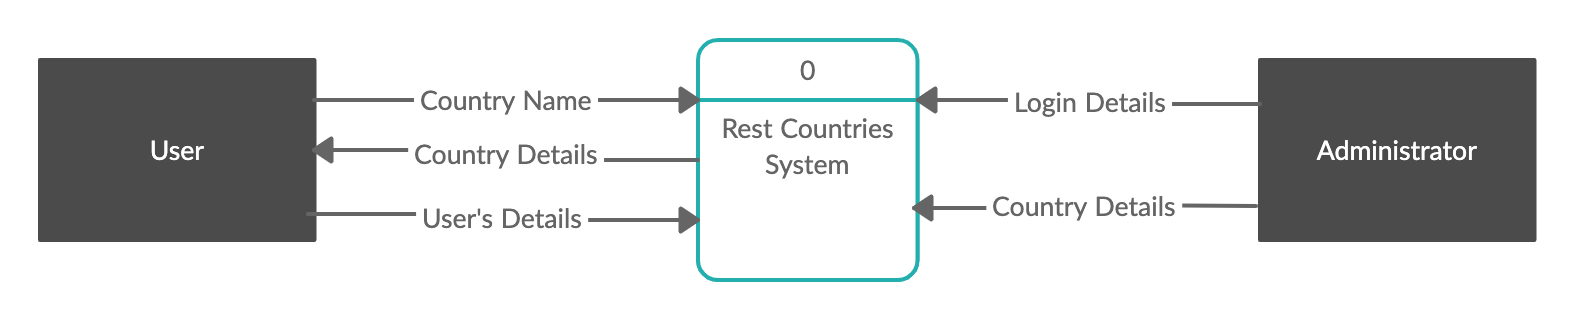
\includegraphics[width=1.0\textwidth]{CFD.png}
	\caption{Context Flow Diagram}
	\label{fig:context-flow-diagram}
\end{figure}

\subsection{Level 1 Data FLow Diagram}
Level 1 DFD is an expansion of the context diagram that shows more processes and how the users interact with the system in terms of inputs and outputs. This is the detailed description of the processes that occur in the system while related to an external entity.

\begin{figure} [h]
	\centering
	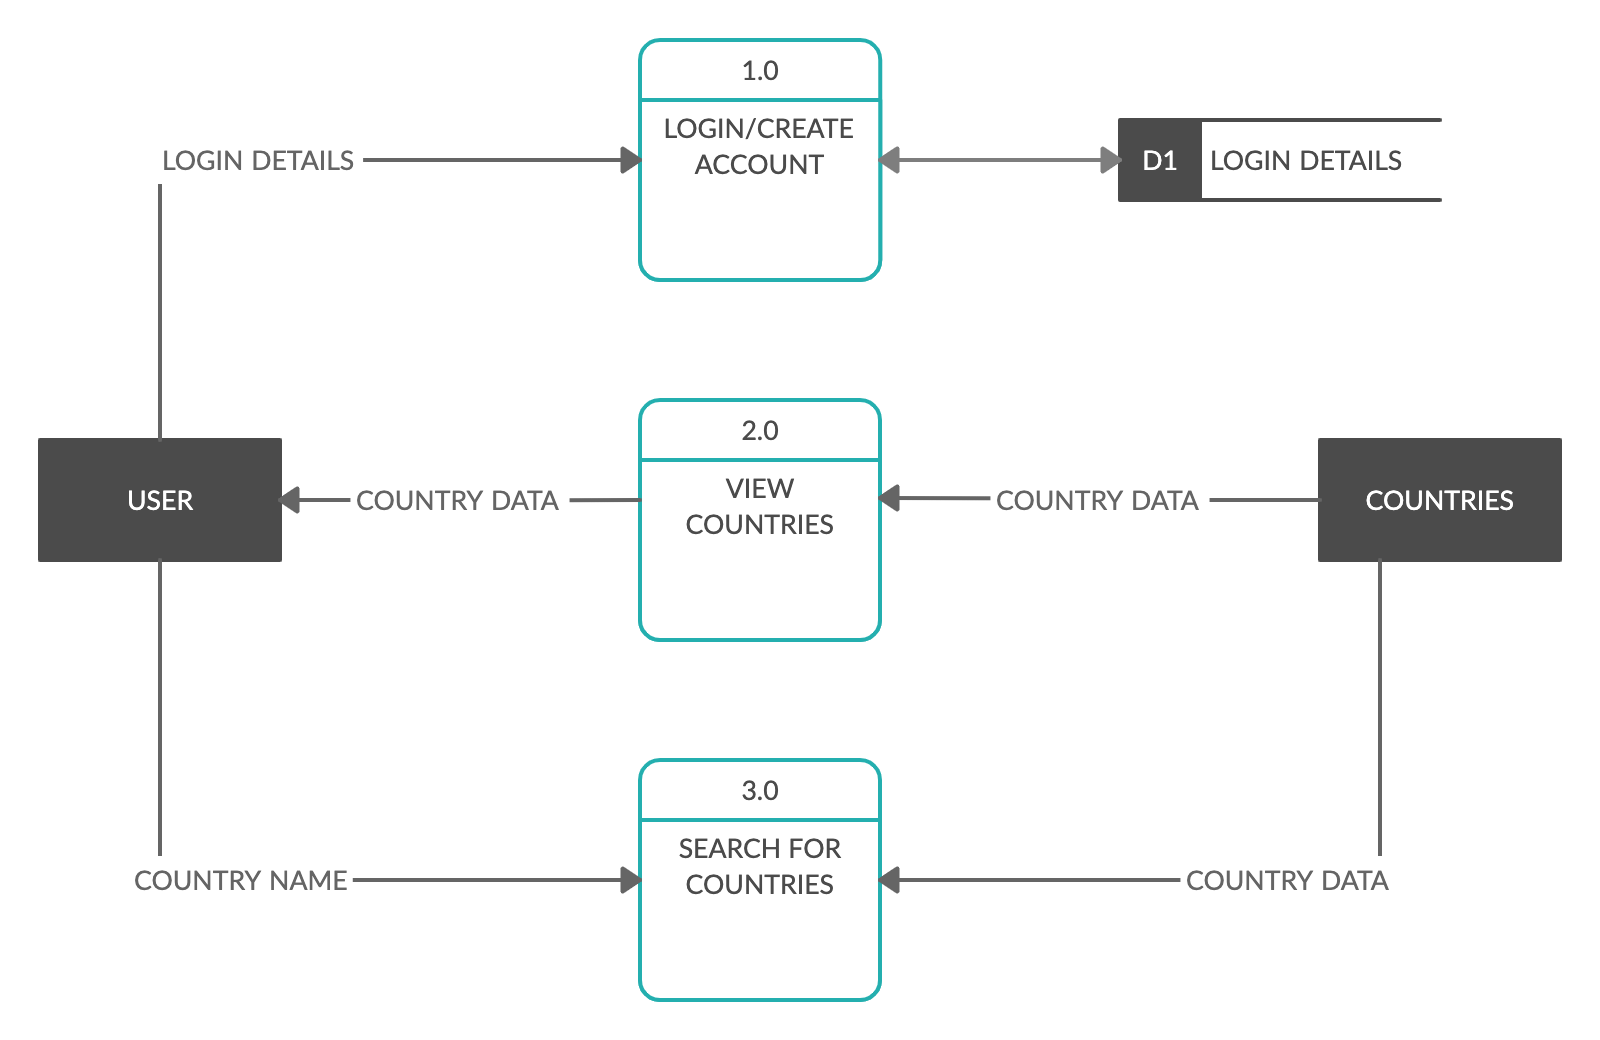
\includegraphics[width=1.0\textwidth]{DFD.png}
	\caption{Level 1 Data Flow Diagram}
	\label{fig:level-1-data-flow-diagram}
\end{figure}

\subsection{Flow Chart}
A flowchart is a type of diagram that represents a work flow or process. They are used in analysing, designing, documenting or managing a process in various fields.\\
\indent
Figure \ref{fig:context-flow-diagram} shows a flowchart representing a systemic flow of how users interact with the system.

\begin{figure}
	\centering
	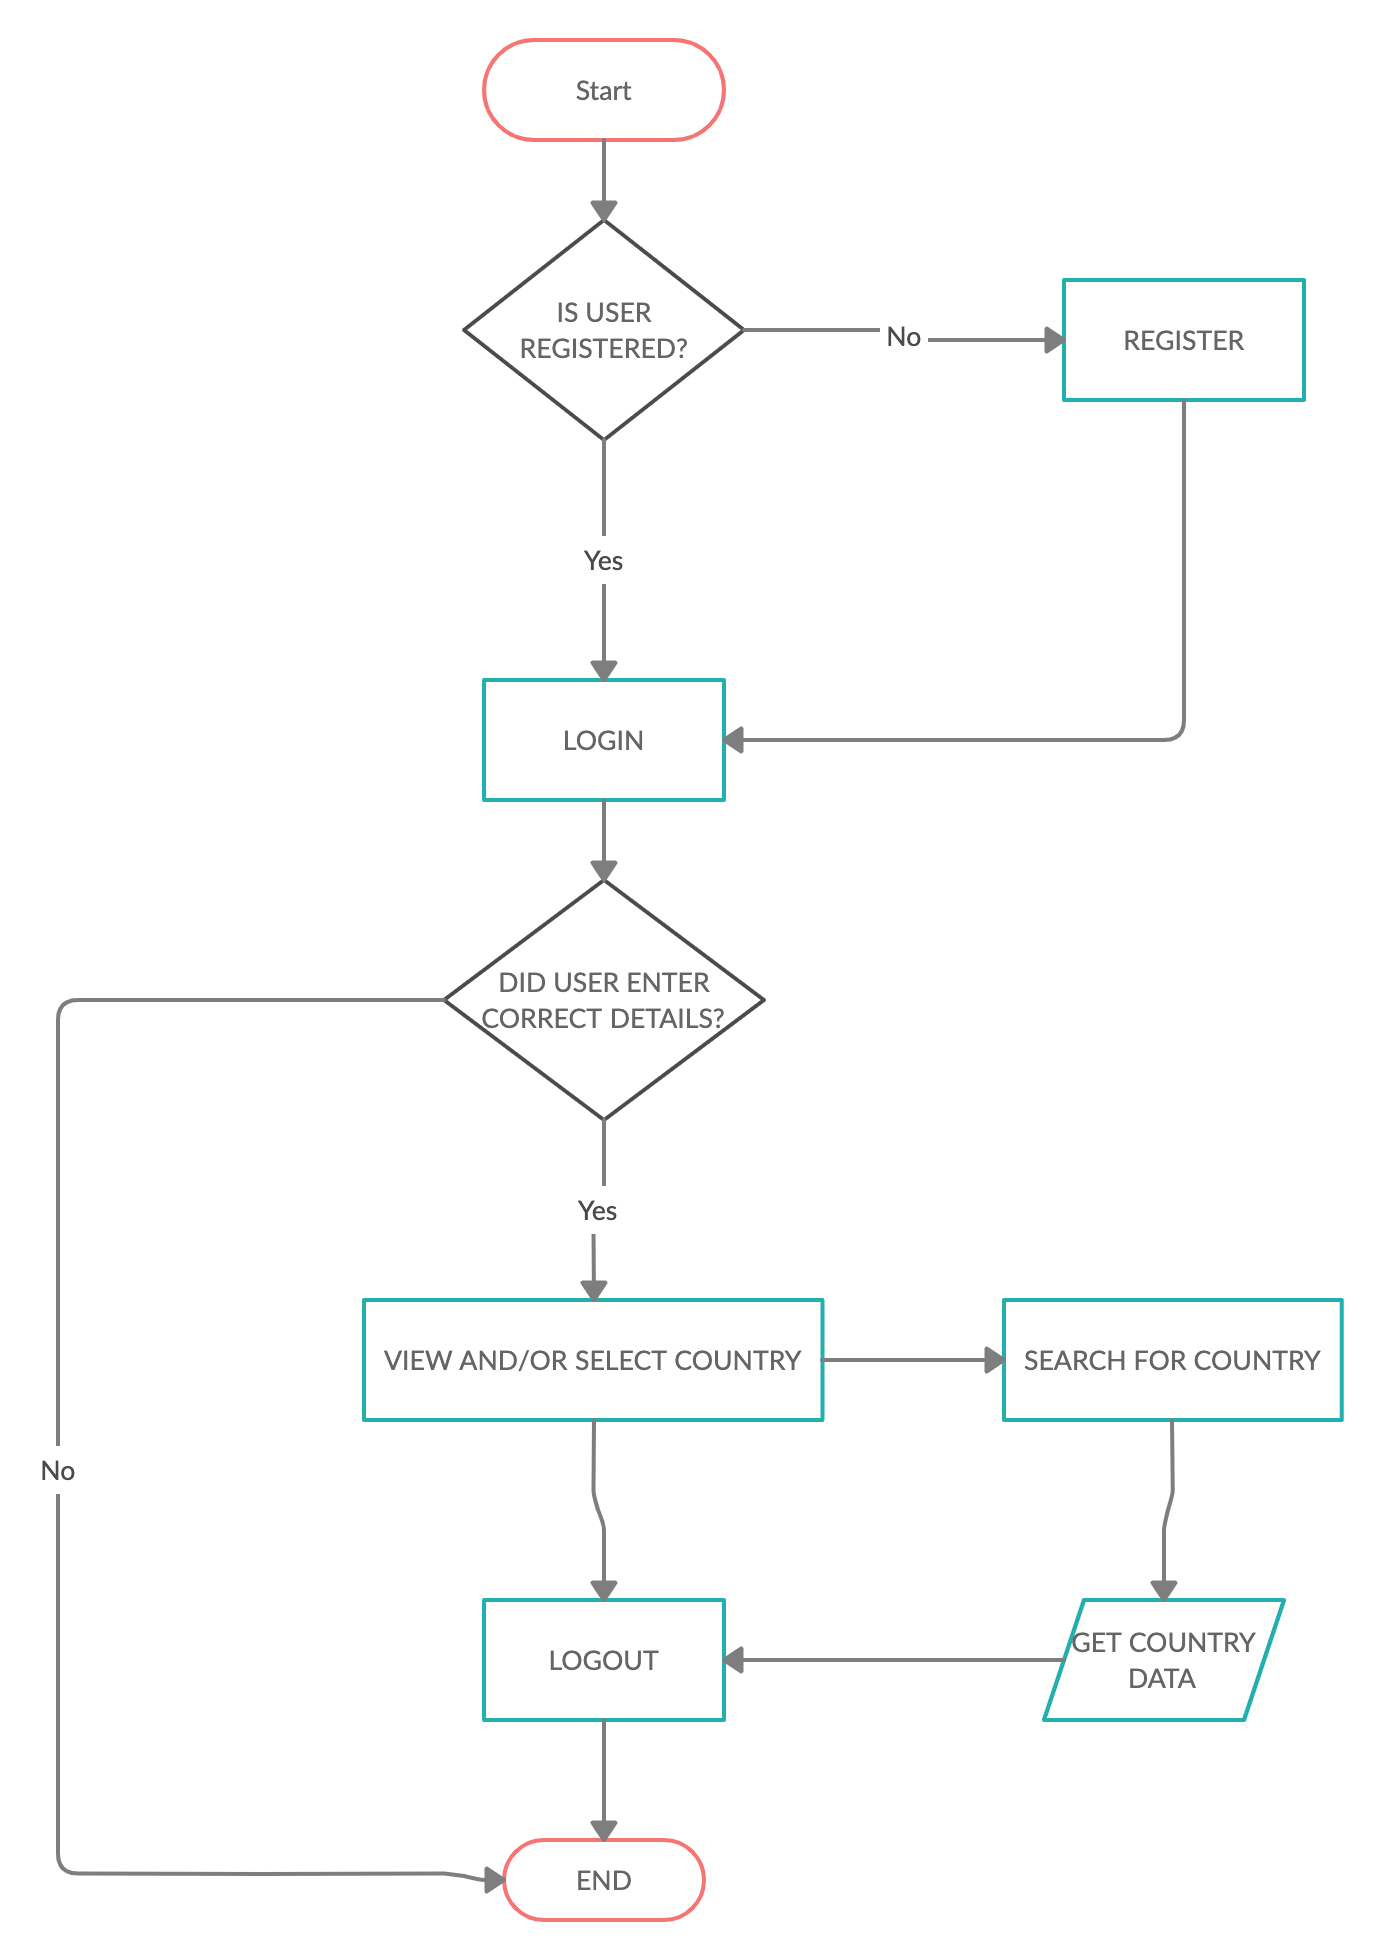
\includegraphics[width=0.9\textwidth]{flowchart.png}
	\caption{Flow Chart Diagram}
	\label{fig:flow-chart-diagram}
\end{figure}

\section{Data Modelling and Entity Relationships}
\subsection{Data Modelling}
A data model is a formal way of representing the data that are used and created by a system; it illustrates people, places, or things about which information is captured and how they are related to each other.\\
\indent
In system design, analysts draw a physical data model to reflect how the data will be physically be stored in the databases and files.

\subsection{Entity Relationship Diagram (ERD)}
An entity relationship diagram is a picture which shows information that is created, stored, and used by a system. On an ERD, similar kinds of information are listed together and placed inside boxes called entities. Lines are drawn between entities to represent relationships among the data, and special symbols are added to the diagram to communicate high-level business rules that need to be supported by the system.

\subsubsection{Entities}
Entities are the basic building blocks of a data model. It is a person, place, event, or thing about which data is collected.\\
The entities in this application include:
\begin{itemize}
	\item Country
	\item Continent
	\item State/Province
	\item Currency
	\item Language
\end{itemize}

\subsubsection{Relationships}
Relationships are associations between entities and they are shown by lines that connect the entities together.
Figure \ref{fig:relationships} below show the description of the various relationships between the entities with their cardinalities.

\begin{figure} [h]
	\centering
	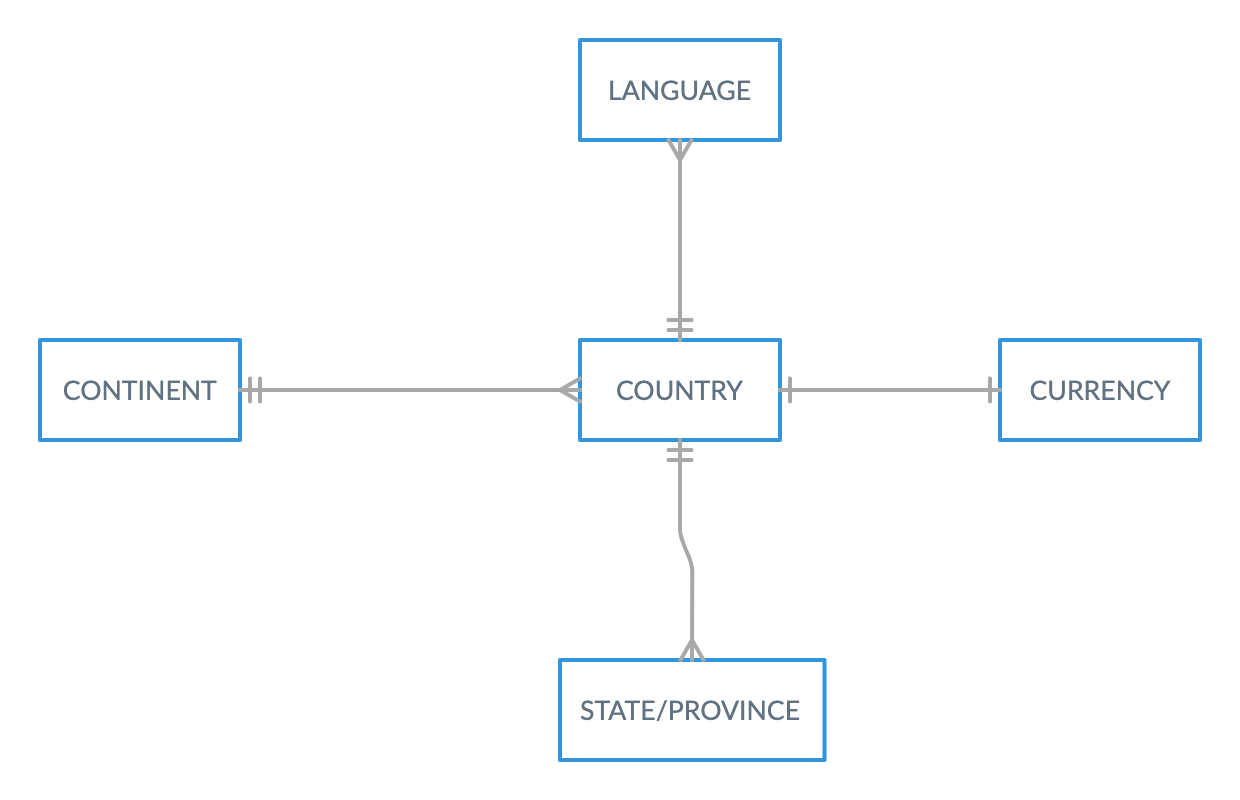
\includegraphics[width=1.0\textwidth]{relationships.png}
	\caption{The Relationships Between the Entities}
	\label{fig:relationships}
\end{figure}

Where:
\begin{itemize}
	\item A Continent has many countries so it represents a One-to-Many Relationship
	\item A Country has many States/Provinces so it represents a One-to-Many Relationship
	\item A Country has only one Currency so it represents a One-to-One relationship
	\item A Country can have one or more Languages so it represents a One-to-Many relationship
\end{itemize}

\begin{figure} [h]
	\centering
	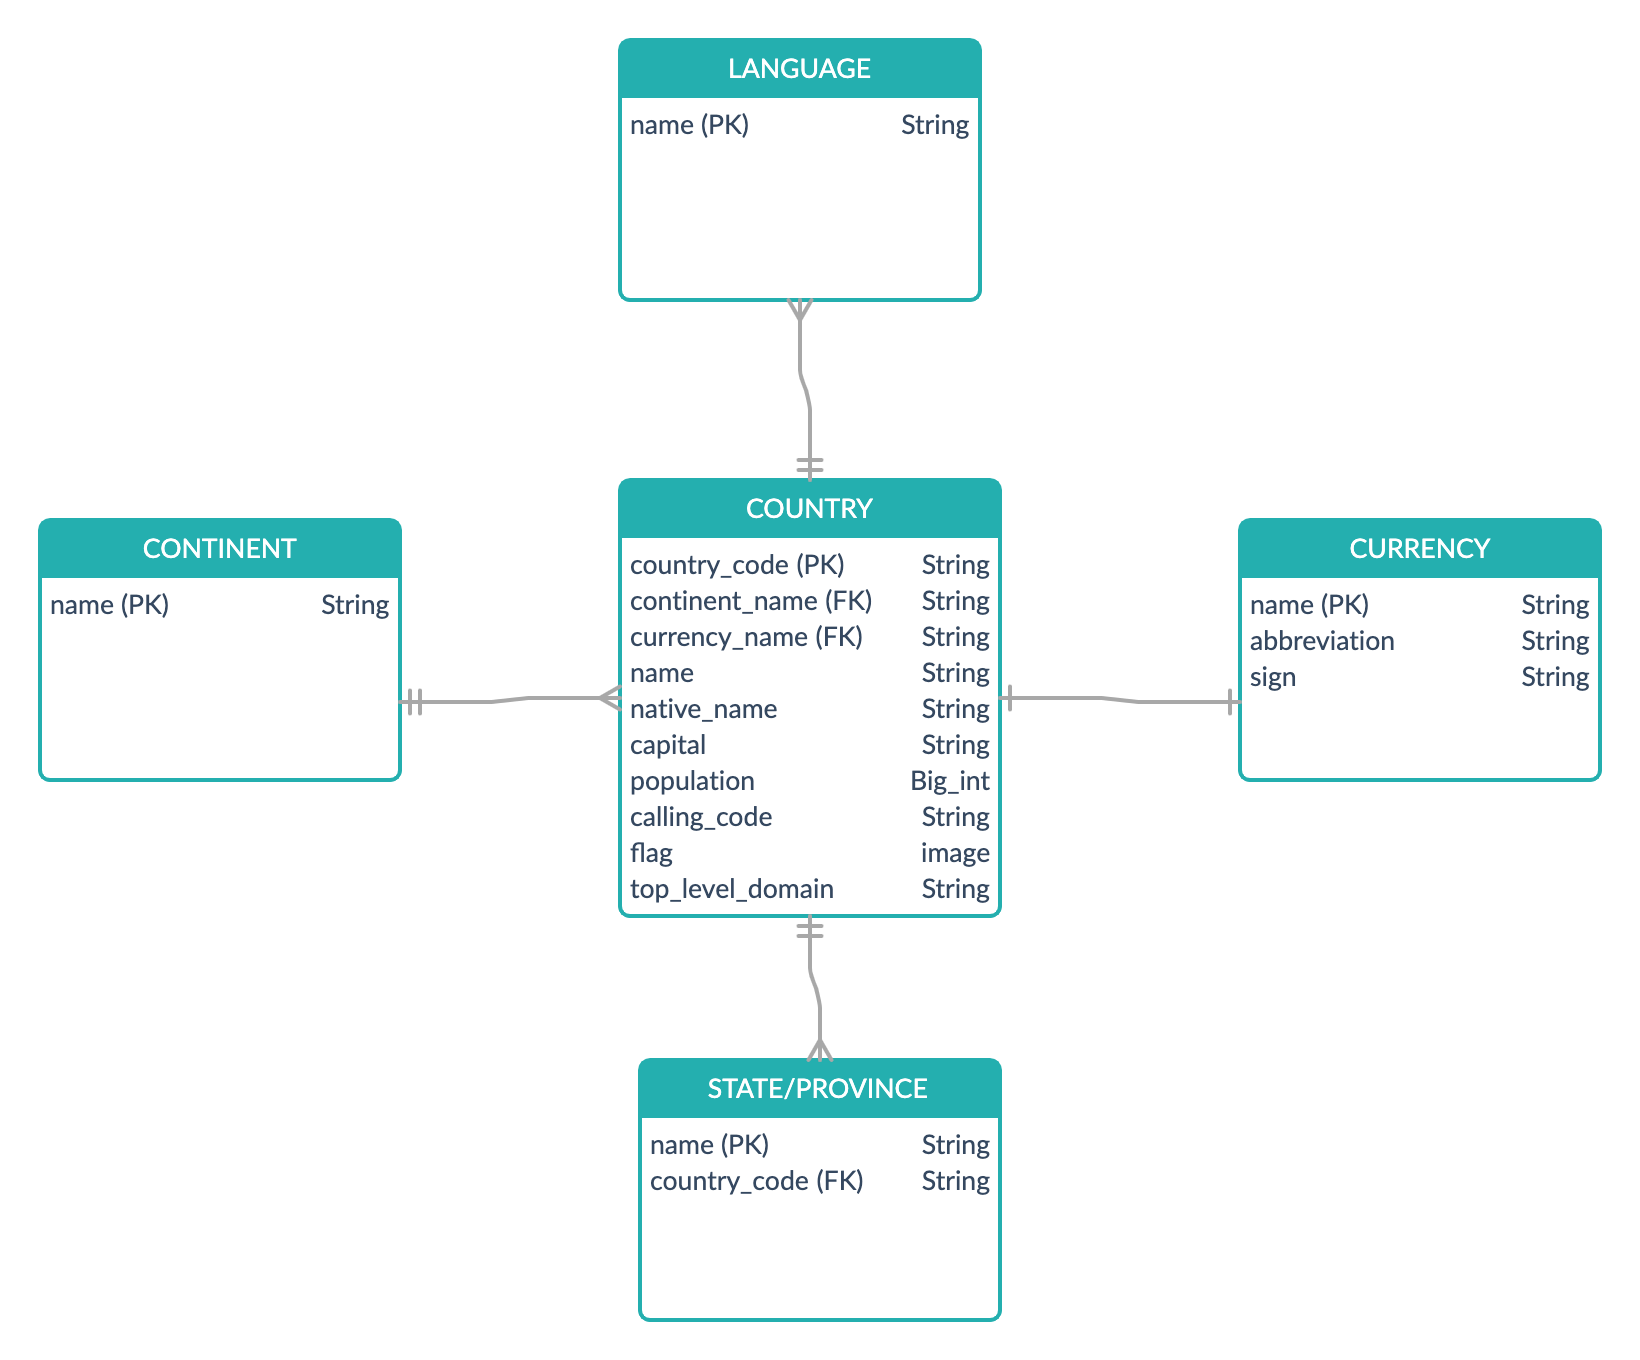
\includegraphics[width=1.0\textwidth]{ERD.png}
	\caption{Entity Relationship Diagram}
	\label{fig:ERD}
\end{figure}

\chapter{Implementation}
\section{Introduction}
Implementation is the stage in the project where the theoretical design is turned into a working system. System implementation is the phase where the application is realised. It involves careful planning, investigation of the current system and its constraints on implementation. The implementation process begins with preparing a plan for the implementation of the system and then proceeds to the activities to be carried out such as creating a mockup or wireframe and then writing the code and then on to the deployment of the application.\\
\indent
Implementation is the final and the most important phase. The most critical stage in acheiving a successful new system is giving the users confidence that the new system will work and be effective. The system can only be implemented after thorough testing is done and it is found to be working according to the specifications.

\section{System Specification}
The application was built based on a REST API called ``REST Countries" which is a simple web API for getting information about the world's nations via REST calls and the API provided the information about the countries in the application.\\ 
\indent
The application was built by mainly using a popular JavaScript framework called \emph{Vue.js}. Vue.js is an open-source front-end JavaScript framework for building interfaces and single-page applications. It features an incrementally adpatable architecture that focuses on declarative rendering and component composition.\\ 
\indent
A state manager called \emph{Vuex} which is the primary state manager for Vue.js was used in the application to store data that was going to be used across the components for easy retrieval. Routing was also implemented in this project to enable the functionality of moving from one page to another and back and it was done mainly using \emph{vue-router} which is the official router for Vue.js. For the styling, \emph{SASS} which is a CSS preprocessor was used to implement the styling of the web application.\\
\indent
Node.js was used together with Express.js to develop the server-side of the application. Node.js which is an open-source, cross-platform, back-end, JavaScript runtime environment that executes JavaScript code outside the browser. Node.js lets developers use JavaScript to write command line tools and for server-side scripting to produce dynamic web page content before the page is sent to the user's browser.\\
\indent
Express.js also referred to as Express, is a free and open-source back-end web application framework for Node.js. It is designed for building web applications and APIs.\\
\indent
MongoDB was used as the database application used to store the user information. MongoDB is a cross-platform document-oriented database program. It is classified as a NoSQL database program, MongoDB uses JSON-like documents with optional schemas.

\section{Description of the User Interface}
The application has the following pages:

\subsection{Login/Register Page}
The application has been designed to ensure that access to the application can only be granted to authenticated users. The user is required to enter a valid username and pasword before access can be granted. Upon entering the right credentials, the user is directed to relevant sections and can now use the application (see Figure \ref{fig:login_page}). If a user is not registered in the system then the user is required to register to have an account so that the user can gain access to the system (see Figure \ref{fig:register_page}).

\begin{figure} 
	\centering
	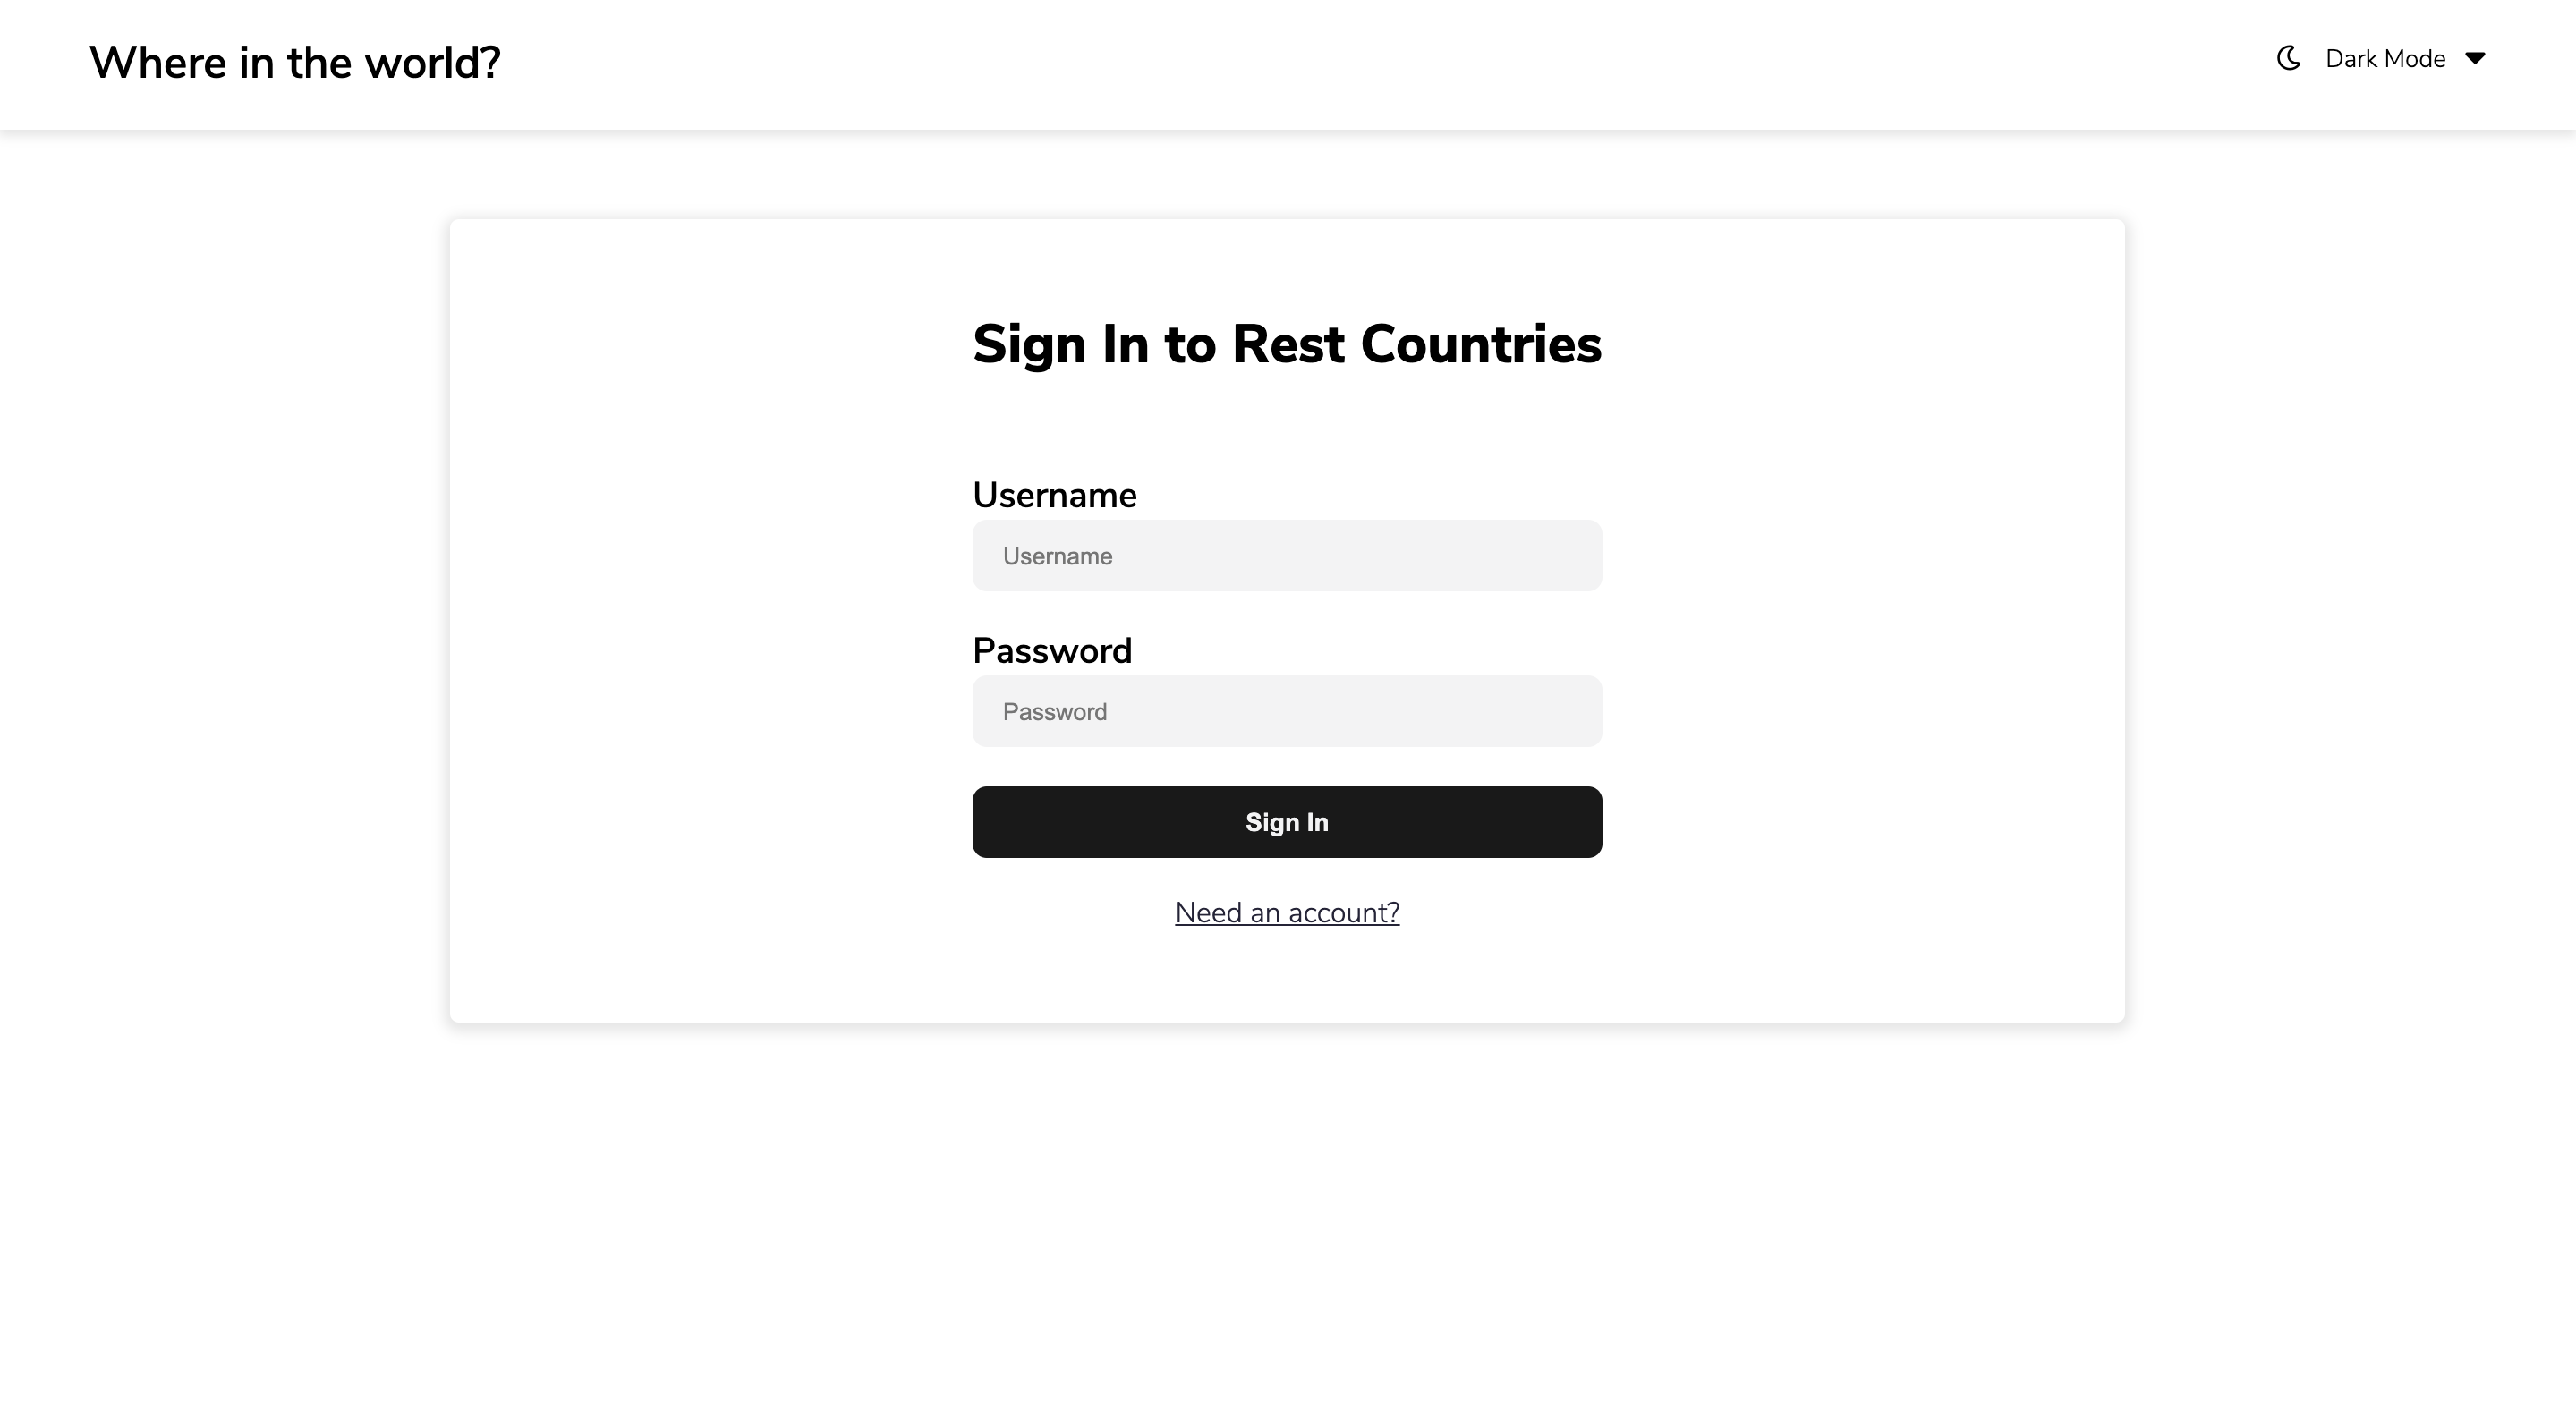
\includegraphics[width=1.0\textwidth]{LoginPage.png}
	\caption{Login Page}
	\label{fig:login_page}
\end{figure}

\begin{figure}
	\centering
	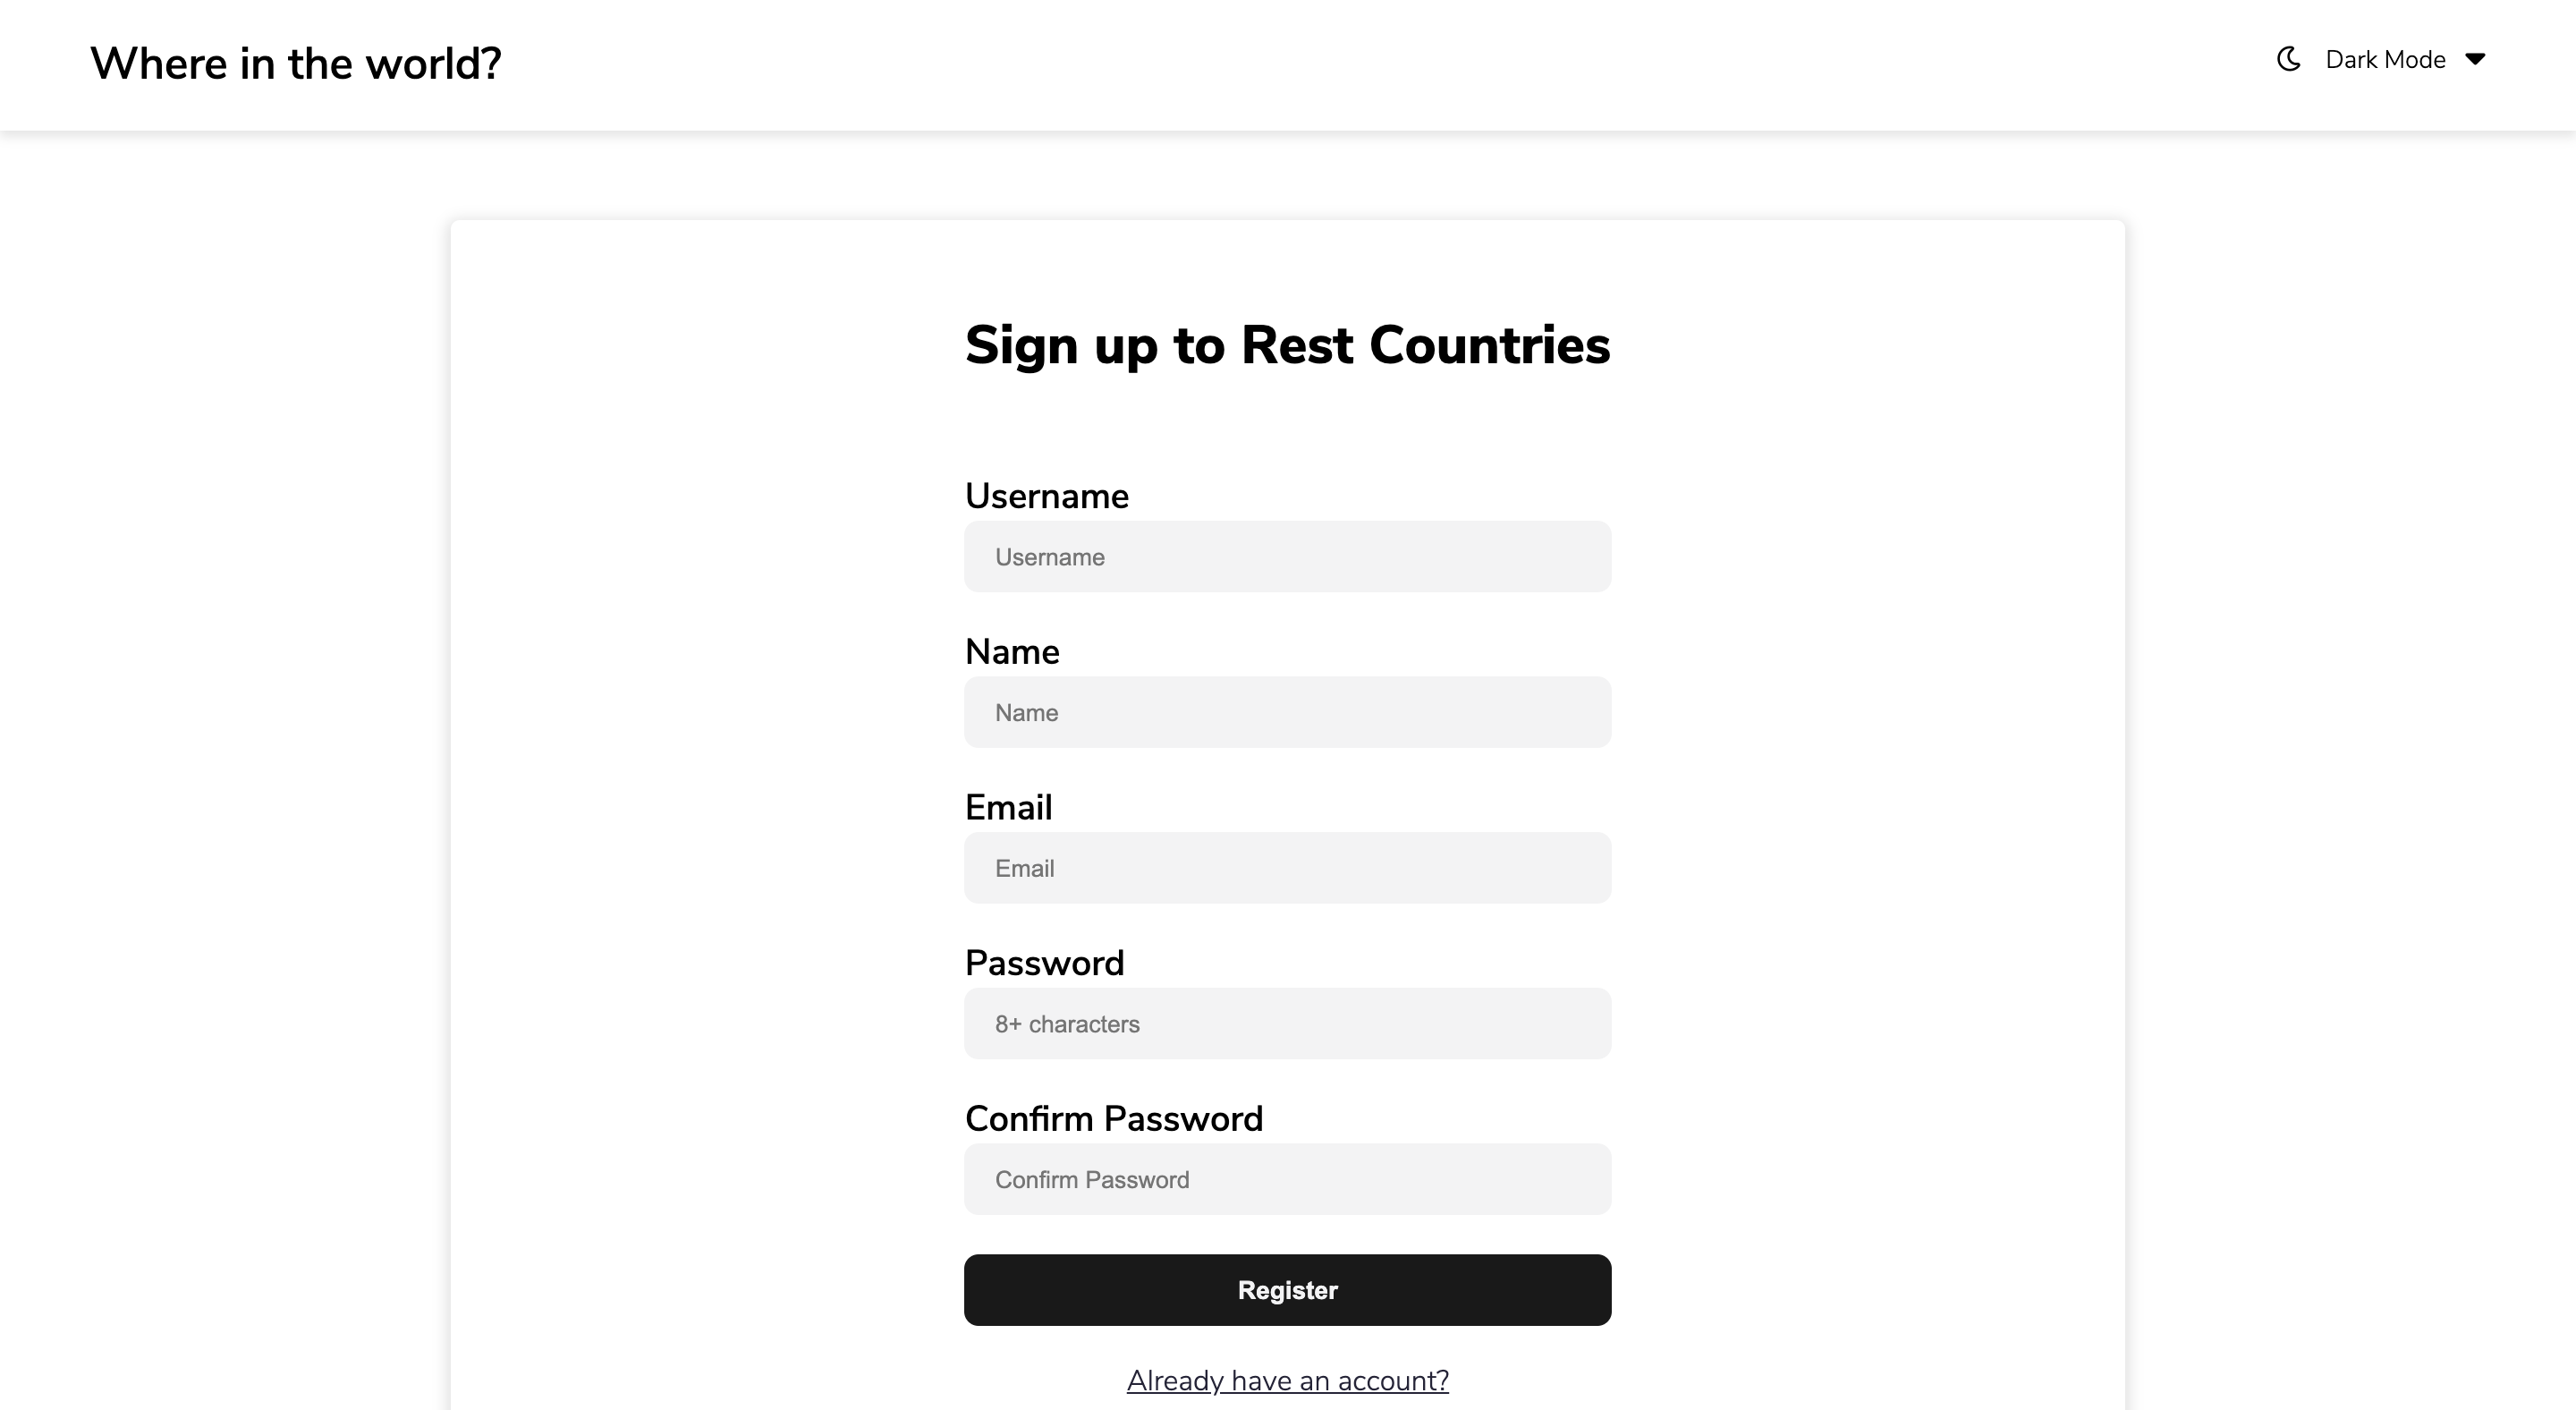
\includegraphics[width=1.0\textwidth]{RegisterPage.png}
	\caption{Register Page}
	\label{fig:register_page}
\end{figure}

\subsection{The Home Page}
The home page displays all the countries in cards. It also features a search box that lets the user type in the name of any country to be searched for and the results are shown in real-time (see Figure \ref{fig:search}). There is also a dropdown feature that enables the user to filter the countries by their continents such as Africa, Asia, etc. (see Figure \ref{fig:home_page})

\begin{figure} [h]
	\centering
	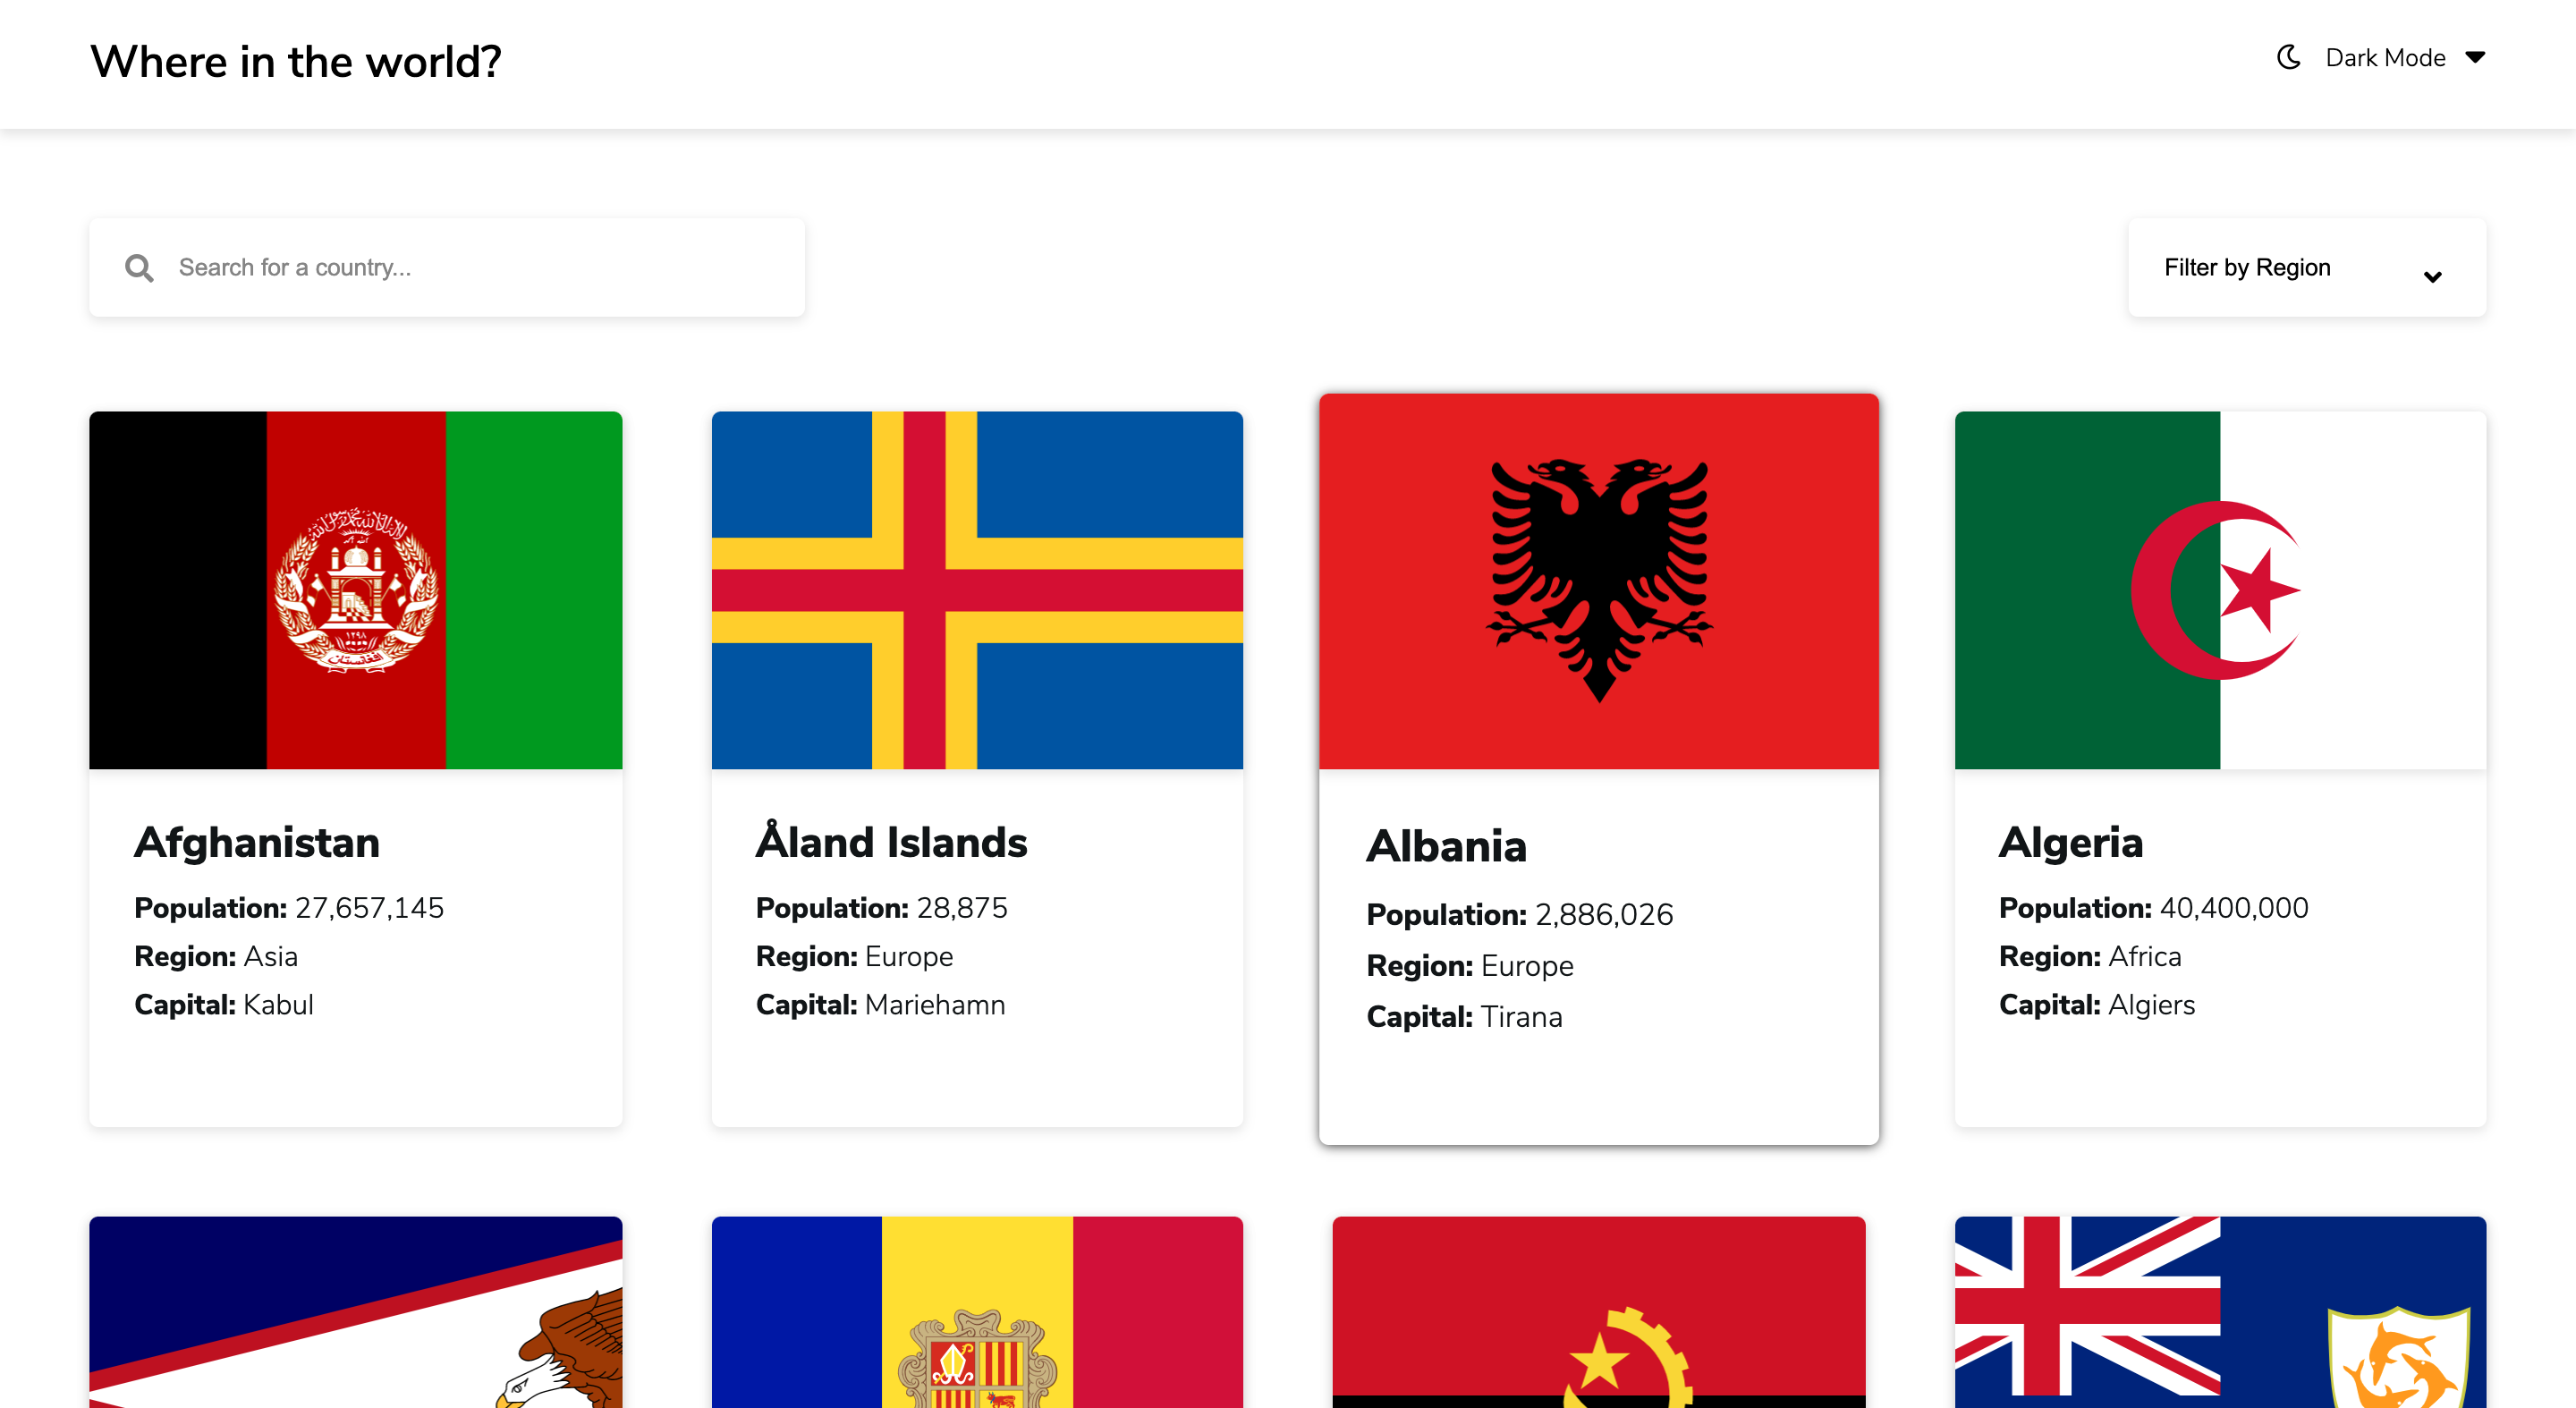
\includegraphics[width=1.0\textwidth]{Home Page.png}
	\caption{Home Page}
	\label{fig:home_page}
\end{figure}

\begin{figure}
	\centering
	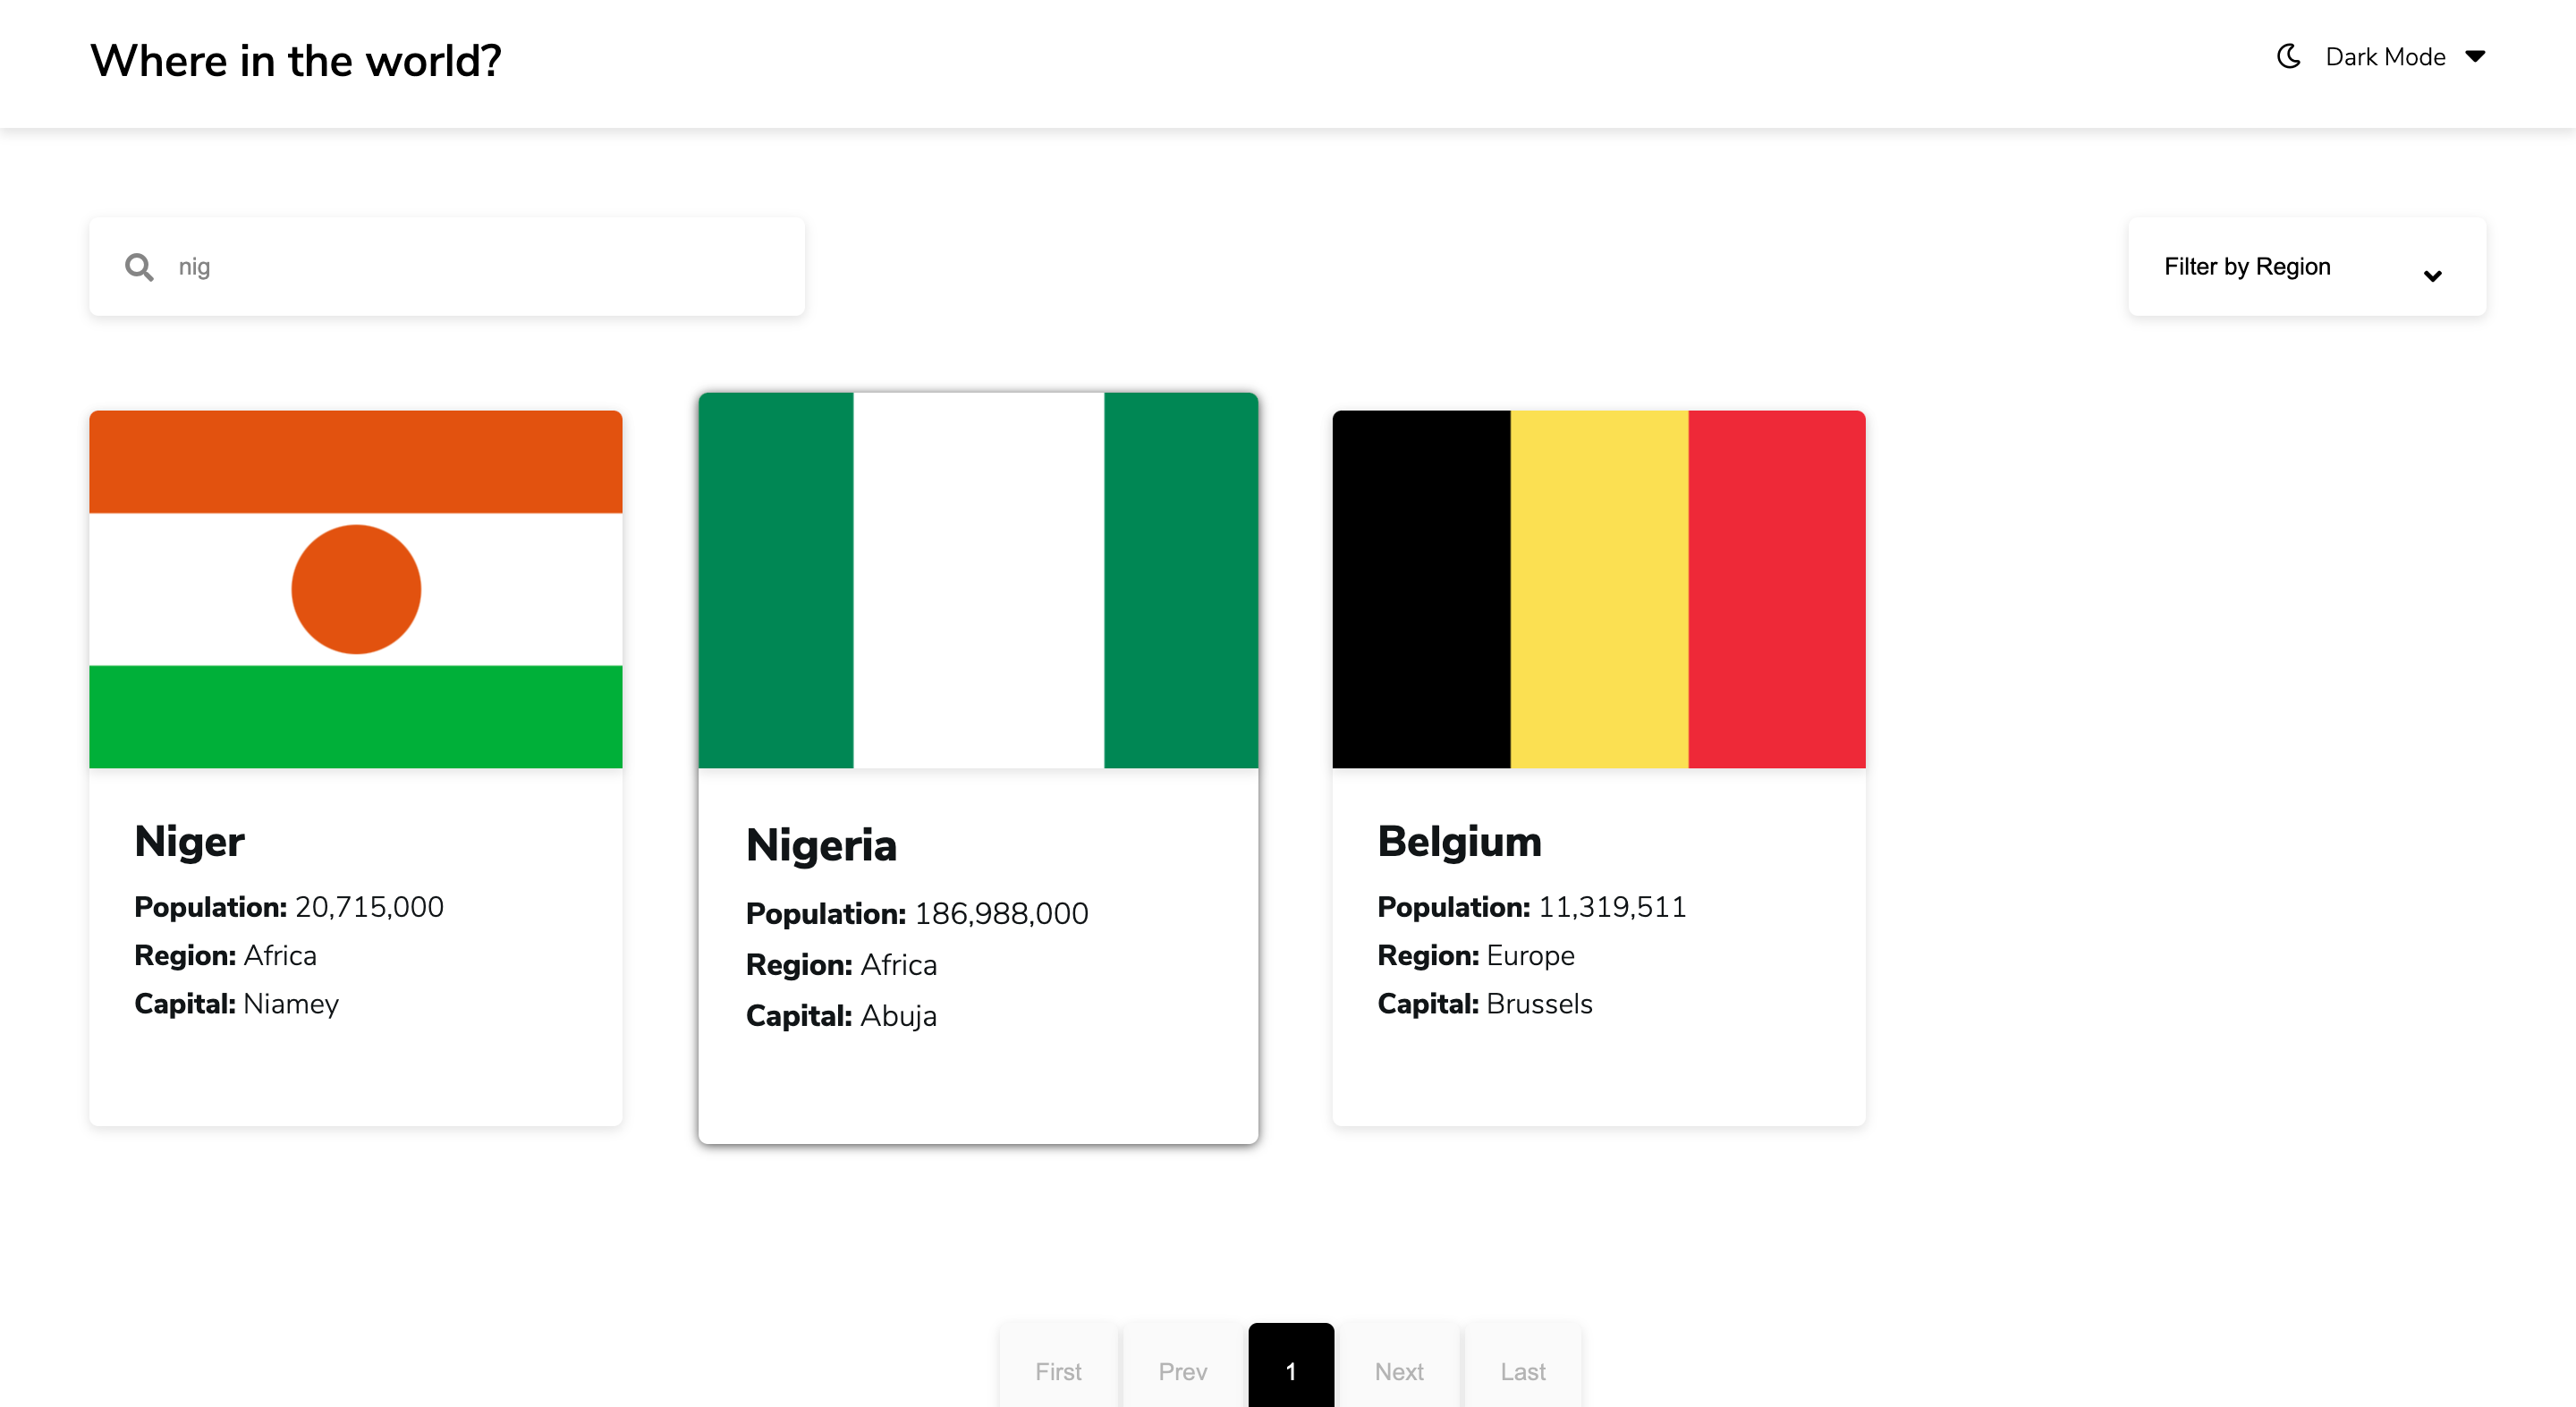
\includegraphics[width=1.0\textwidth]{search.png}
	\caption{Home Page}
	\label{fig:search}
\end{figure}

\subsection{The Descriptions Page}
When a card on the home page is clicked, the user is automatically redirected to the descriptions page and this page displays the full information about the particular country that was selected (see Figure \ref{fig:descriptions_page}).

\begin{figure}
	\centering
	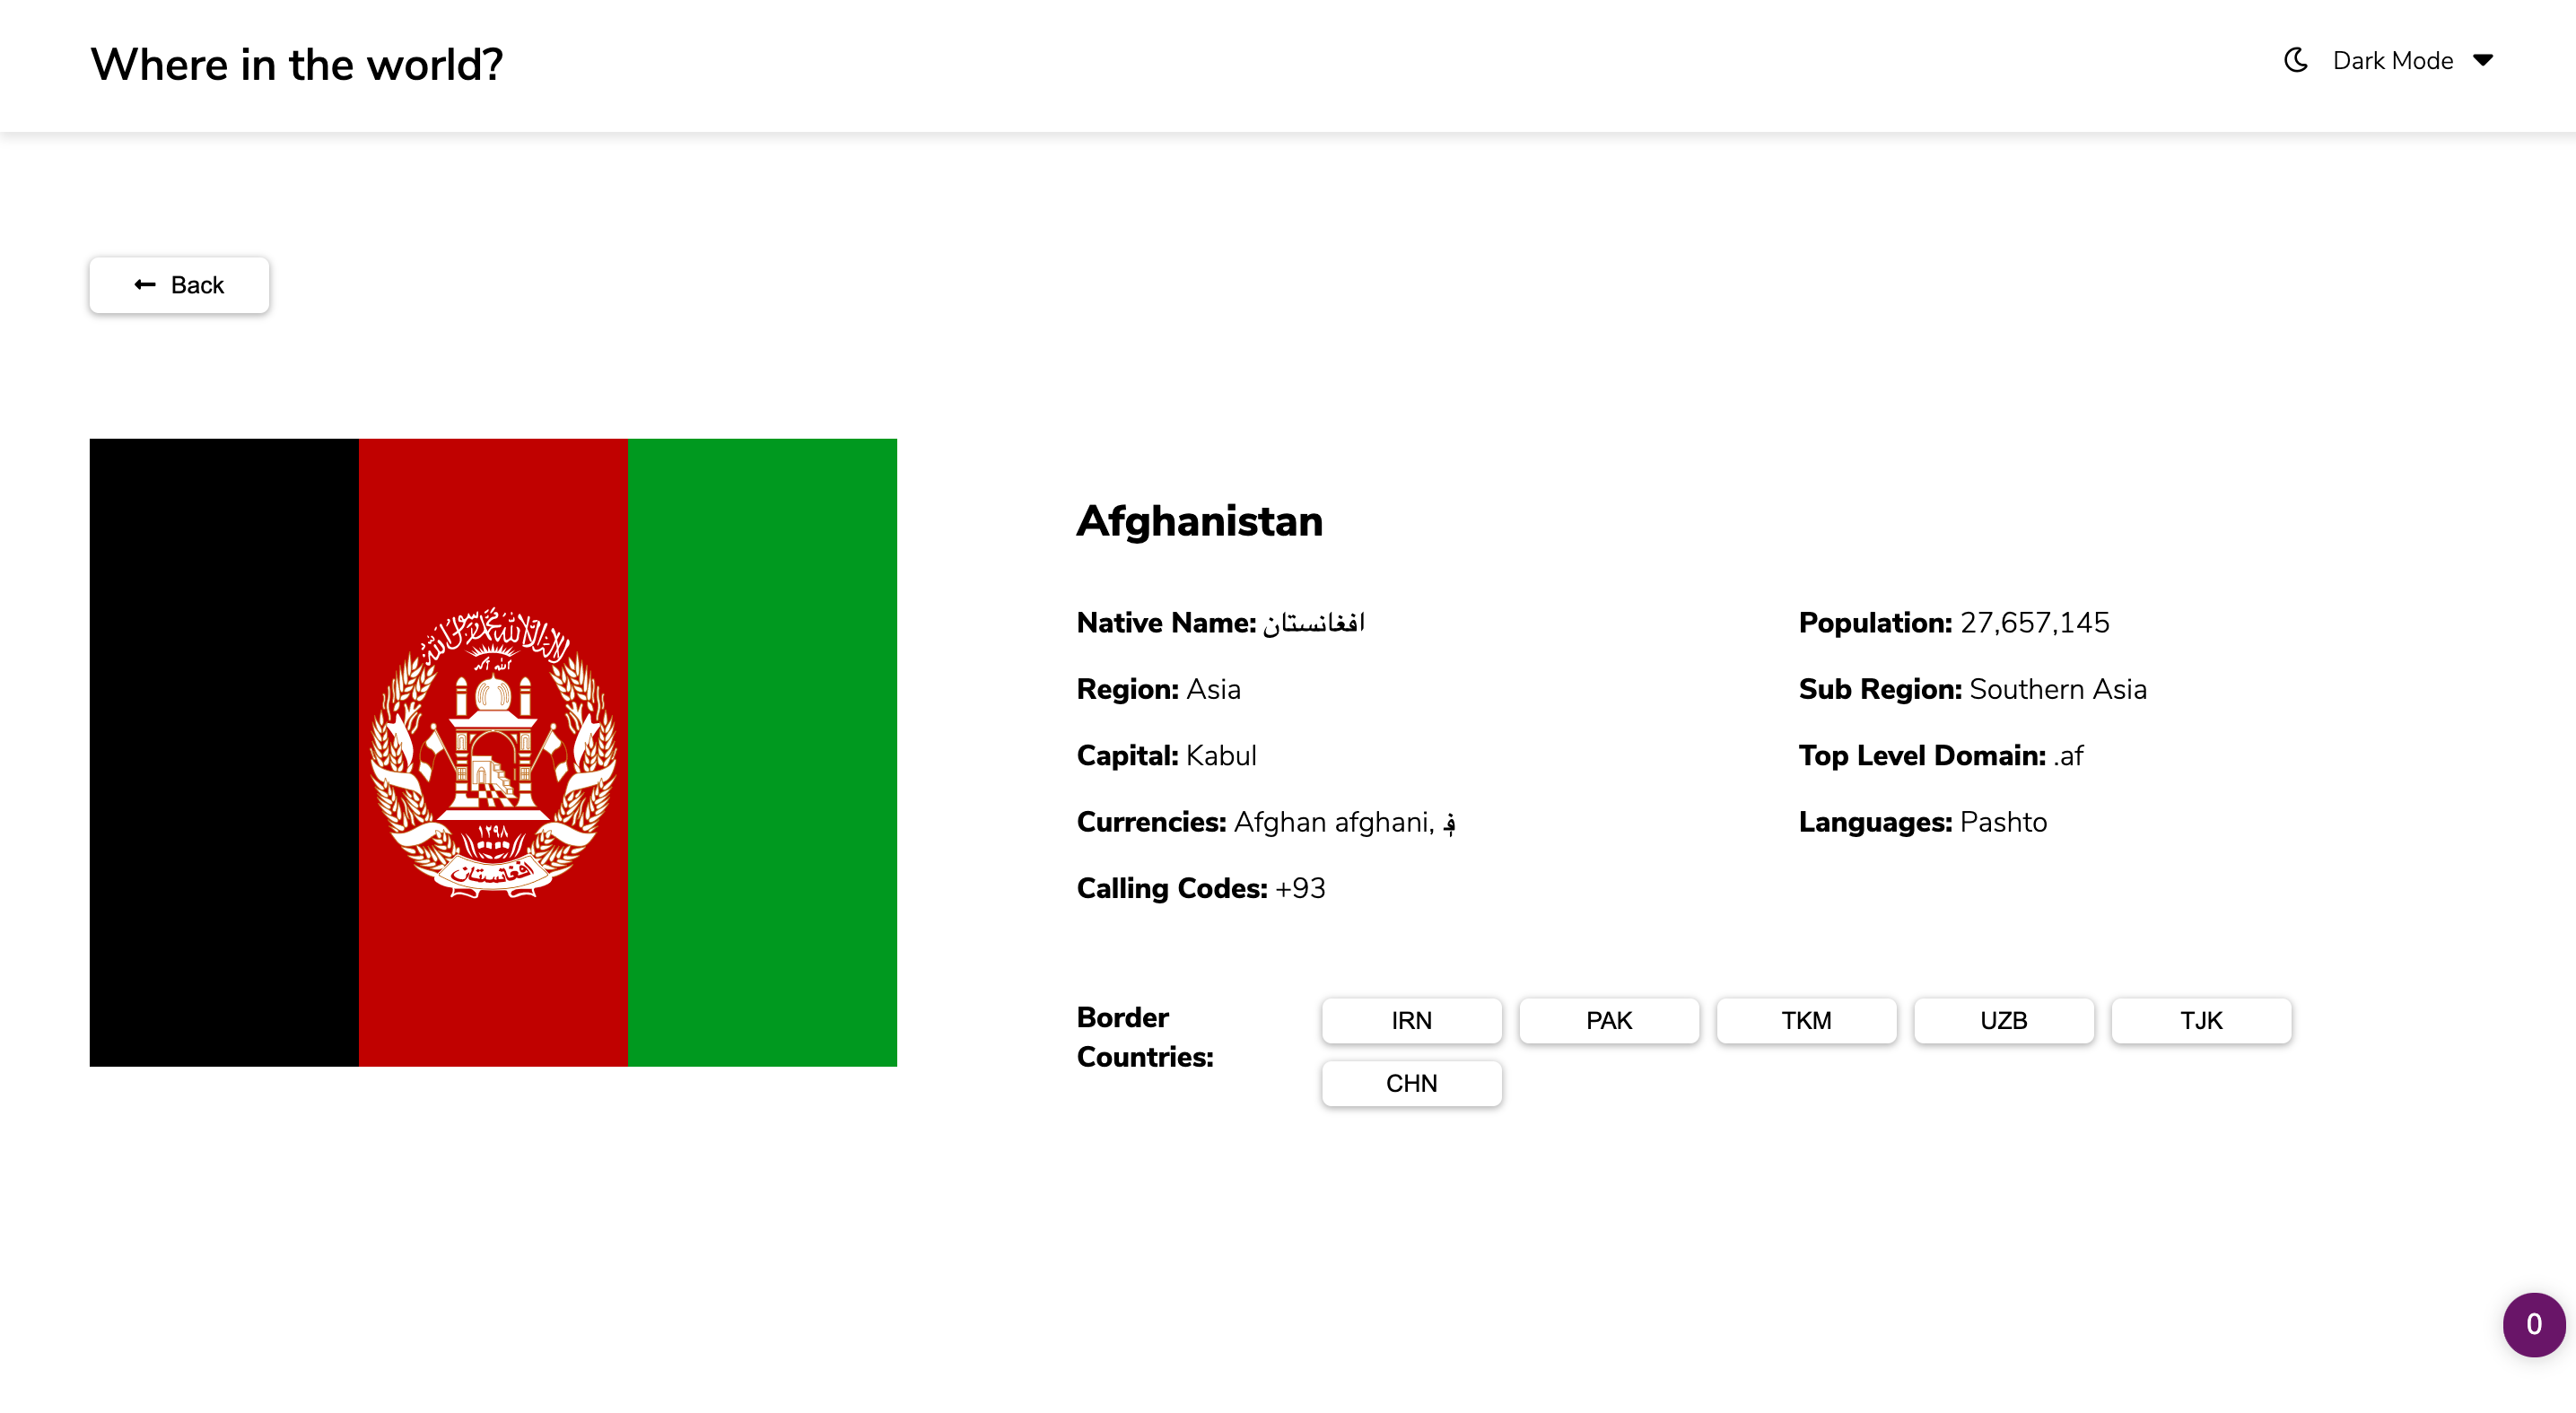
\includegraphics[width=1.0\textwidth]{DescriptionsPage.png}
	\caption{Descriptions Page}
	\label{fig:descriptions_page}
\end{figure}

\subsection{Colour Switcher}
The application also features a colour switcher which enables the user to toggle a colour switch to change the the design theme of the application from light mode to dark mode (see Figure \ref{fig:darkmode}).

\begin{figure} [h]
	\centering
	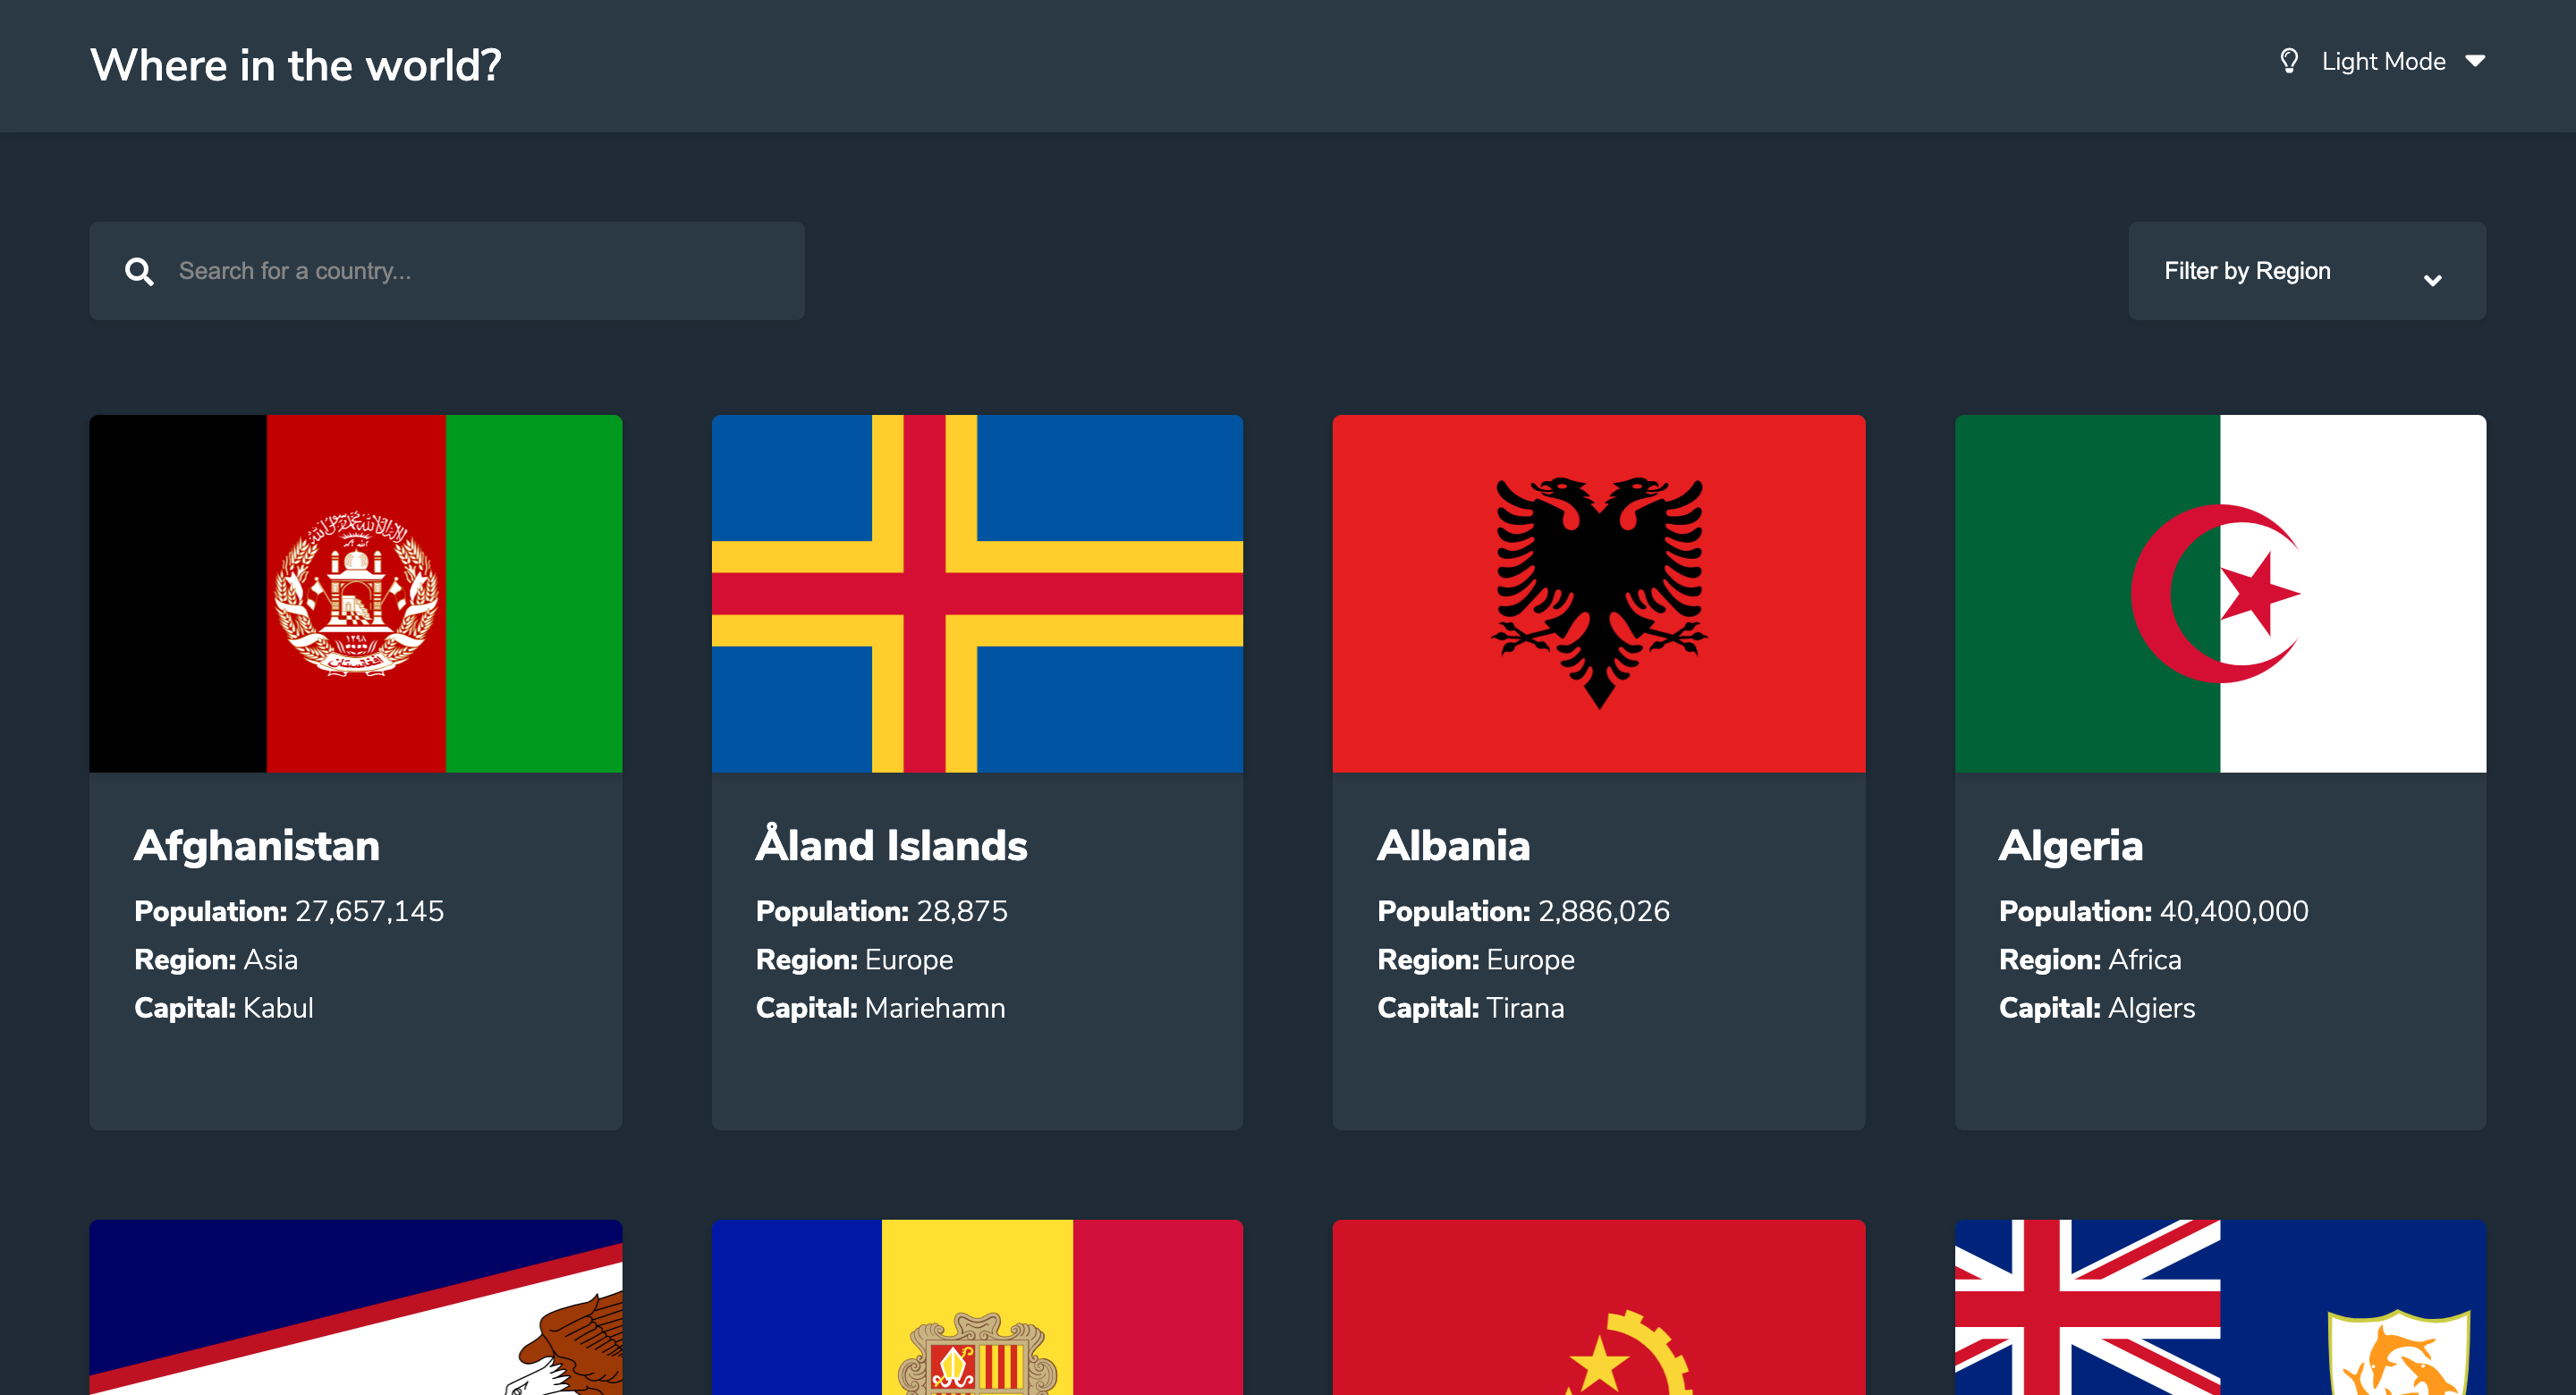
\includegraphics[width=1.0\textwidth]{darkmode.png}
	\caption{Application in Dark Mode}
	\label{fig:darkmode}
\end{figure}

\section{Implementing Interactivity}
This chapter focus primarily on the system implementation phase of the system development process. One of the main concerns of the implementation phase is the interface design. Therefore it is important that the interface is designed in a way that it eases user to accomplish their task by interacting with the system efficiently and effectively. A well designed interface possesses the ability to attract and change user’s perception towards a system. In this project, the system interfaces were designed by considering various interactive design elements as to promote the better interaction of user and the system.

\printbibliography

\end{document}